Multi-jet production is a source of background in the \hadhad SR in which both
\tauhadvis candidates originate from the misidentification of quark- or
gluon-initiated jets. It represents the second-largest background with
\faketauhadvis in the \hadhad SR after the dominant \ttbarFakes contribution.

\subsubsection{The Fake Factor Method}

The multi-jet background is estimated using the data-driven fake factor
method. It is applicable in cases where two observables exist that are
statistically independent for the background process to be estimated while also
being strong discriminators between the background and other processes (i.e.\
signal and non-multi-jet processes). Four disjoint regions can be defined, three
background-enriched CRs and a signal-like region, by categorising events based
on both observables. The assumption of statistical independence allows relating
the expected number of events for the background process between CRs and the
signal-like region. This can be used to estimate the background in the
signal-like region using data observed in the CRs.

In the \hadhad channel, two observables that allow to define CRs enriched in
multi-jet events are the \tauid requirements fulfilled by the \tauhadvis
candidates and the sign of the electric charges of both candidates. Two disjoint
regions are defined based on the \tauid requirement: the ID~region and the
\antiid~region. The ID~region consists of events in which both \tauhadvis
candidates pass the loose \tauid working point. The identification criterion is
partially inverted to define a multi-jet enriched CR by requiring exactly one
loose \tauhadvis and exactly one
anti-\tauhadvis~(cf.~\Cref{sec:object_reconstruction}). This region is referred
to as the \antiid~region. Similarly, two regions are defined based on the charge
signs of the two \tauhadvis candidates: an OS~region and a SS~region. Lastly,
the \tauid and charge sign criterion are combined to define four distinct
regions: the OS~ID~region (the signal-like region), the OS~Anti-ID~region, the
SS~ID~region, and the SS~Anti-ID~region.

% In the SR, \tauhadvis candidates are required to pass the loose \tauid working
% point. This requirement defines regions where both \tauhadvis candidates pass
% identification, hereafter referred to as ID regions. The selection is
% partially inverted to obtain CRs enhanced in multi-jet events by requiring
% that exactly one \tauhadvis candidate is failing the loose \tauid working
% point while still passing a working point corresponding to a true \tauhadvis
% identification efficiency of about \SI{99}{\percent}
% ($\text{RNN score} > 0.01$). The \tauhadvis candidates fulfilling this
% selection are referred to as anti-\tauhadvis and the regions defined by the
% inversion of the identification criterion as Anti-ID regions. The
% identification criterion cannot be fully inverted due to a pre-selection
% applied in the data reduction pipeline of the ATLAS
% experiment.\footnote{Datasets targeting $\PHiggs \to \hadhad$ require events
% with at least one \tauhadvis passing the loose \tauid working point and one
% \tauhadvis with a \tauid score exceeding 0.01.}  However, the fake factor
% method is still valid in the presence of these constraints provided the
% underlying assumptions of the method hold.

% The electric charge of \tauhadvis candidates produced in signal or backgrounds
% processes with two \tauhadvis from hadronic decays of \tauleptons (e.g.\
% $\PZ \to \tautau$, $\PHiggs \to \tautau$, \ttbar) are expected to be
% reconstructed with opposite-sign (OS). The OS requirement is inverted yielding
% regions with \tauhadvis candidates of same-sign (SS) electric charge,
% depleting the region of processes where both \tauhadvis originate from
% hadronic \taulepton decays. In contrast, the multi-jet background contributes
% similarly to the OS and SS regions since \tauhadvis charge reconstruction has
% little sensitivity to the relative sign of the electric charge between a pair
% of partons initiating jets that are misidentified as \tauhadvis.

With these region definitions and the independence assumption, the expected
multi-jet contribution in the OS ID region can be estimated according to
\begin{align*}
  N_\text{multi-jet}^{\text{OS, ID}} =
  N_\text{multi-jet}^{\text{OS, Anti-ID}}
  \cdot
  \underbrace{\frac{N_\text{multi-jet}^{\text{SS, ID}}}
  {N_\text{multi-jet}^{\text{SS, Anti-ID}}}}
  _{\eqqcolon \text{FF}_{\text{SS}}} \,\text{,}
\end{align*}
where $N_\text{multi-jet}^{r}$ is the expected number of multi-jet events in
region~$r$. The ratio of multi-jet events in the ID and Anti-ID region is
referred to as the fake factor (FF).
% \footnote{The use of identification or isolation criteria to defining the
% ratio is the main difference between the fake factor method and the more
% general ABCD method.}
Generally, the CRs do not provide pure samples of multi-jet events, and thus the
number of multi-jet events has to be estimated according to
\begin{align*}
  N_\text{multi-jet}^{r} = N_\text{data}^{r} - N_\text{non-multi-jet}^{r} \,\text{,}
\end{align*}
where $N_\text{data}^{r}$ is the observed number of events in region~$r$ and
$N_\text{non-multi-jet}^{r}$ the expected number of non-multi-jet events in
region~$r$ estimated using simulation. Lastly, the probability of misidentifying
a quark- or gluon-initiated jet as a \tauhadvis depends on the properties of the
reconstructed \tauhadvis candidate, especially on \Ntracks and \pT. To control
for this effect, FFs are measured in bins of \tauhadvis candidate properties.

% In addition, the probability of misidentifying a quark- or gluon-initiated jet
% as a \tauhadvis depends on the properties of the reconstructed \tauhadvis
% candidate. Particularly, the reconstructed decay mode and visible transverse
% momentum affect the probability of a jet reconstructed as a \tauhadvis to pass
% \tauid. To control for this effect, FFs are measured in bins of \tauhadvis
% candidate properties.

In~\Cref{tab:mjfakes_yields} the expected multi-jet and non-multi-jet event
yields in the regions relevant for the \faketauhadvis estimation are
summarised. The 2 $b$-tag region, while most similar to the SR, is not well
suited to estimate FFs:
\begin{itemize}

\item The 2 $b$-tag regions relevant for the FF measurement have large
  contributions from non-multi-jet sources, primarily \ttbarFakes, that have to
  be subtracted. The large size of the subtraction leads to a degradation of the
  statistical precision of the FFs and an increase in systematic uncertainties
  from modelling uncertainties on the subtracted components.

\item The strict \btag requirement suppresses the multi-jet contribution in the
  CRs preventing a measurement of FFs in bins of \tauhadvis candidate
  properties.

\item The multi-jet estimate cannot be validated in the 2 $b$-tag region due to
  the absence of a region with high multi-jet purity that is similar to the SR.

\end{itemize}
These issues are partially addressed by performing the FF measurement in the 1
$b$-tag region, which has a higher abundance and purity of multi-jet events, and
extrapolating the measurement to the 2 $b$-tag region to obtain a multi-jet
background estimate in the SR. Distributions of the \pT of the leading and
sub-leading \tauhadvis candidates in the regions relevant to the FF measurement
are shown in~\Cref{fig:mjfakes_1tag_ss_plots}.

\begin{table}[htbp]
  \centering

  \caption{Expected number of multi-jet and non-multi-jet events in regions
    entering the FF method in the \hadhad channel. The expected number of
    multi-jet events is estimated by subtracting the expected number of
    non-multi-jet events from the observed number of events in a given
    region. The breakdown is shown after the 1 $b$-tag requirement in (a); after
    the 2 $b$-tag requirement in (b). The SR (2 $b$-tag OS ID) is omitted. Only
    statistical uncertainties on the expected event yields are shown.}%
  \label{tab:mjfakes_yields}

  \begin{subtable}[t]{\textwidth}
    \centering

    \subcaption{1 $b$-tag regions}
    \label{tab:mjfakes_yields_1tag}

    % Size of subtraction and multi-jet purity:
%                         multi_jet  non_multi_jet  multi_jet_error  non_multi_jet_error  multi_jet_purity
% anti_id charge_sign
% False   OS           16067.048497   16443.951503       204.558258            96.607872          0.494203
%         SS           14040.394005    1971.605995       129.147367            25.827164          0.876867
% True    OS           91582.182374   13677.817626       334.090987            79.729466          0.870057
%         SS           78399.983641    5707.016359       296.470480            61.544664          0.932146

\begin{tabular}{
  ll
  S[table-format=5.0(3)]
  S[table-format=5.0(3)]
  c}
  \toprule
  \multicolumn{2}{l}{Region} & {$N_\text{multi-jet}$} & {$N_\text{non-multi-jet}$} & {Multi-jet purity} \\
  \midrule
  \multirow{2}{*}{SS} & ID      & 14040 +- 130 & 1970 +- 30   & 88\,\% \\
                      & Anti-ID & 78400 +- 300 & 5710 +- 70   & 93\,\% \\
  \midrule
  \multirow{2}{*}{OS} & ID      & 16070 +- 210 & 16440 +- 100 & 49\,\% \\
                      & Anti-ID & 91580 +- 340 & 13680 +- 80  & 87\,\% \\
  \bottomrule
\end{tabular}



%%% Local Variables:
%%% mode: latex
%%% TeX-master: "../phd_thesis"
%%% End:

  \end{subtable}

  \vspace{11pt}

  \begin{subtable}[t]{\textwidth}
    \centering

    \subcaption{2 $b$-tag regions}

    % Size of subtraction and multi-jet purity:
%                        multi_jet  non_multi_jet  multi_jet_error  non_multi_jet_error  multi_jet_purity
% anti_id charge_sign
% False   OS            408.197943    7971.802057       105.950917            53.344135          0.048711
%         SS           1299.622259    1001.377741        50.345854            15.287412          0.564808
% True    OS           8429.603396    8864.396604       139.699303            47.136984          0.487429
%         SS           7653.735896    3338.264104       108.557939            28.157166          0.696301

\begin{tabular}{
  ll
  S[table-format=5.0(3)]
  S[table-format=5.0(3)]
  c}
  \toprule
  \multicolumn{2}{l}{Region} & {$N_\text{multi-jet}$} & {$N_\text{non-multi-jet}$} & {Multi-jet purity} \\
  \midrule
  \multirow{2}{*}{SS} & ID      & 1300 +- 60  & 1000 +- 20 & 56\,\% \\
                             & Anti-ID & 7650 +- 110 & 3340 +- 30 & 70\,\% \\
  \midrule
  \multirow{2}{*}{OS} & ID      & \multicolumn{3}{c}{\rule[3pt]{5.2em}{0.3pt}\hspace{1em}Signal Region\hspace{1em}\rule[3pt]{5.2em}{0.3pt}} \\
                             & Anti-ID & 8430 +- 140 & 8860 +- 50 & 49\,\% \\
  \bottomrule
\end{tabular}




%%% Local Variables:
%%% mode: latex
%%% TeX-master: "../phd_thesis"
%%% End:

  \end{subtable}
\end{table}

\begin{figure}[htbp]
  \centering

  \begin{subfigure}{0.49\textwidth}
    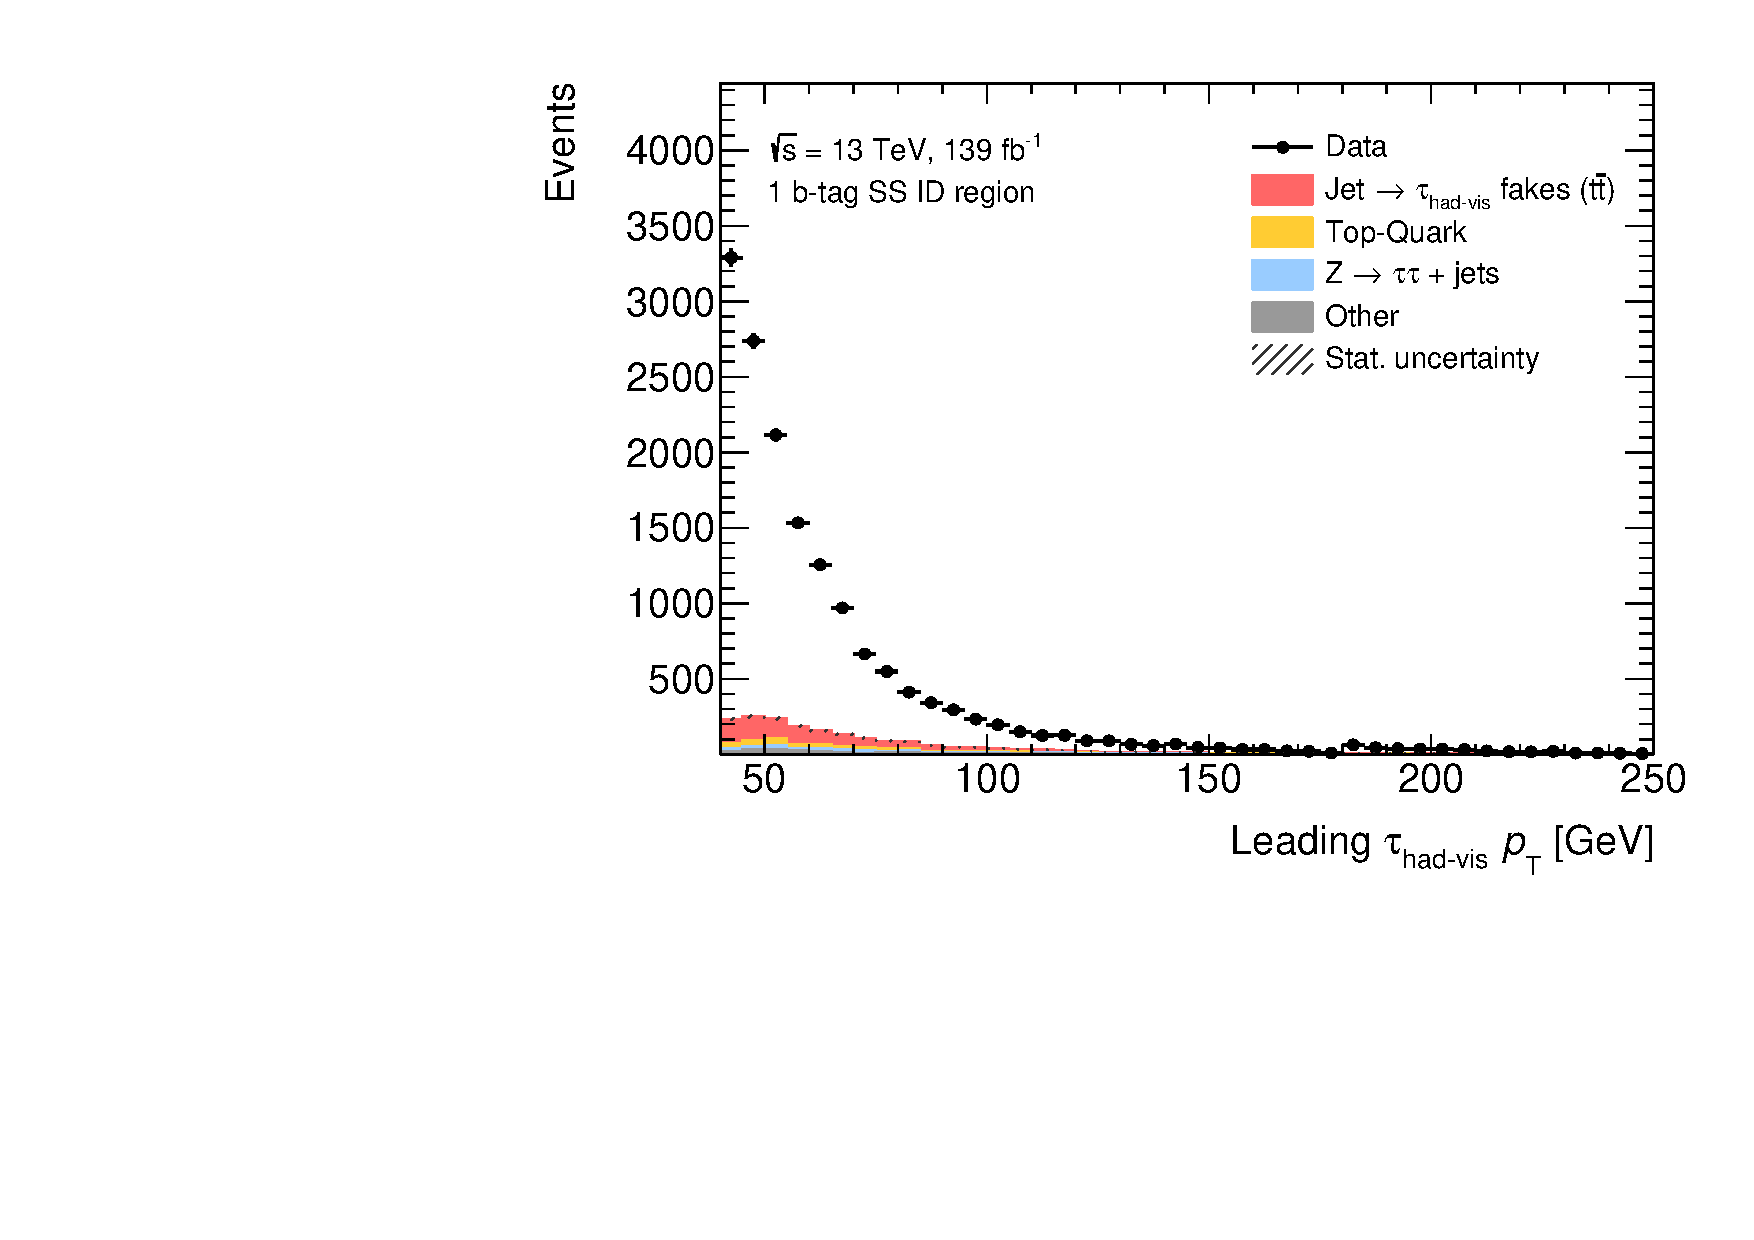
\includegraphics[width=\textwidth]{fakefactors/region_plots/tau0pt_1tag_ss_id}
    \subcaption{1 $b$-tag SS ID region}
  \end{subfigure}
  \begin{subfigure}{0.49\textwidth}
    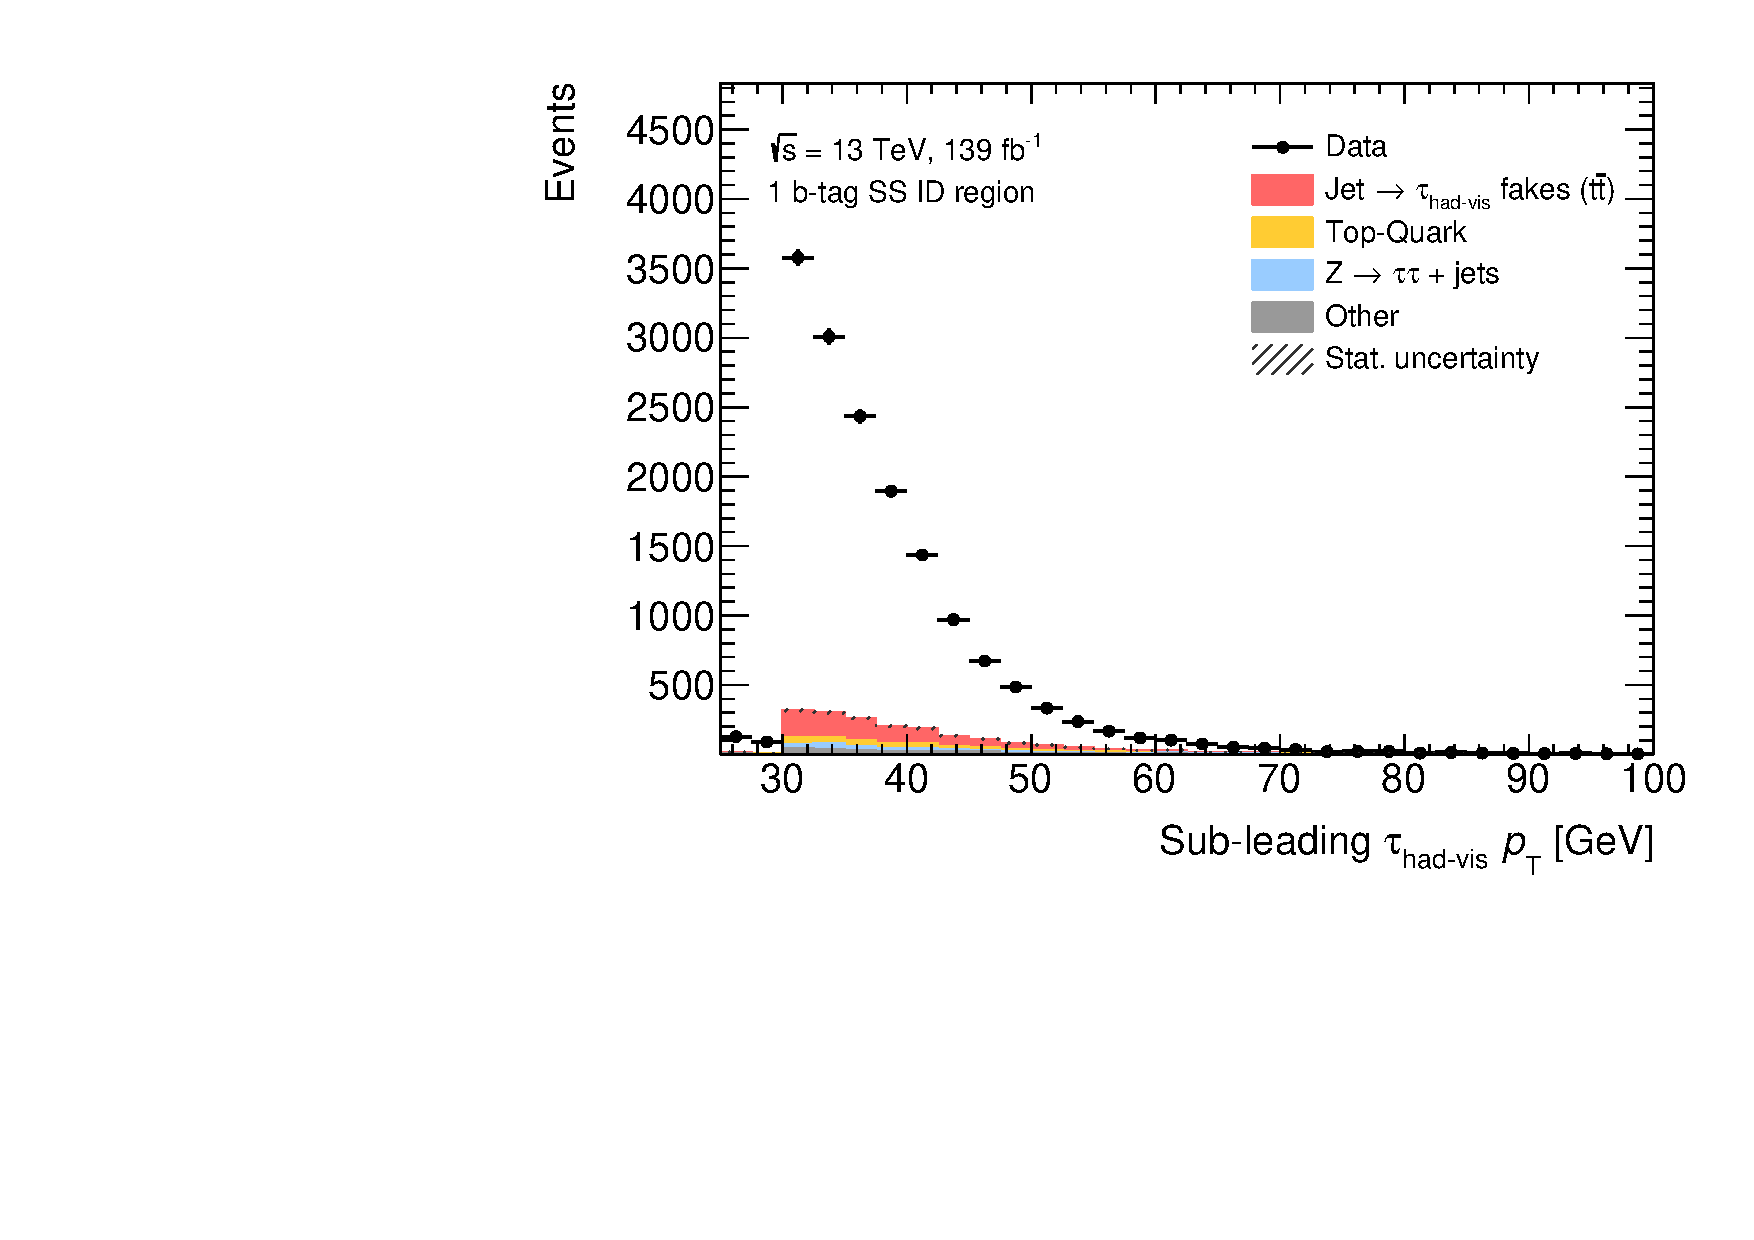
\includegraphics[width=\textwidth]{fakefactors/region_plots/tau1pt_1tag_ss_id}
    \subcaption{1 $b$-tag SS ID region}
  \end{subfigure}

  \begin{subfigure}{0.49\textwidth}
    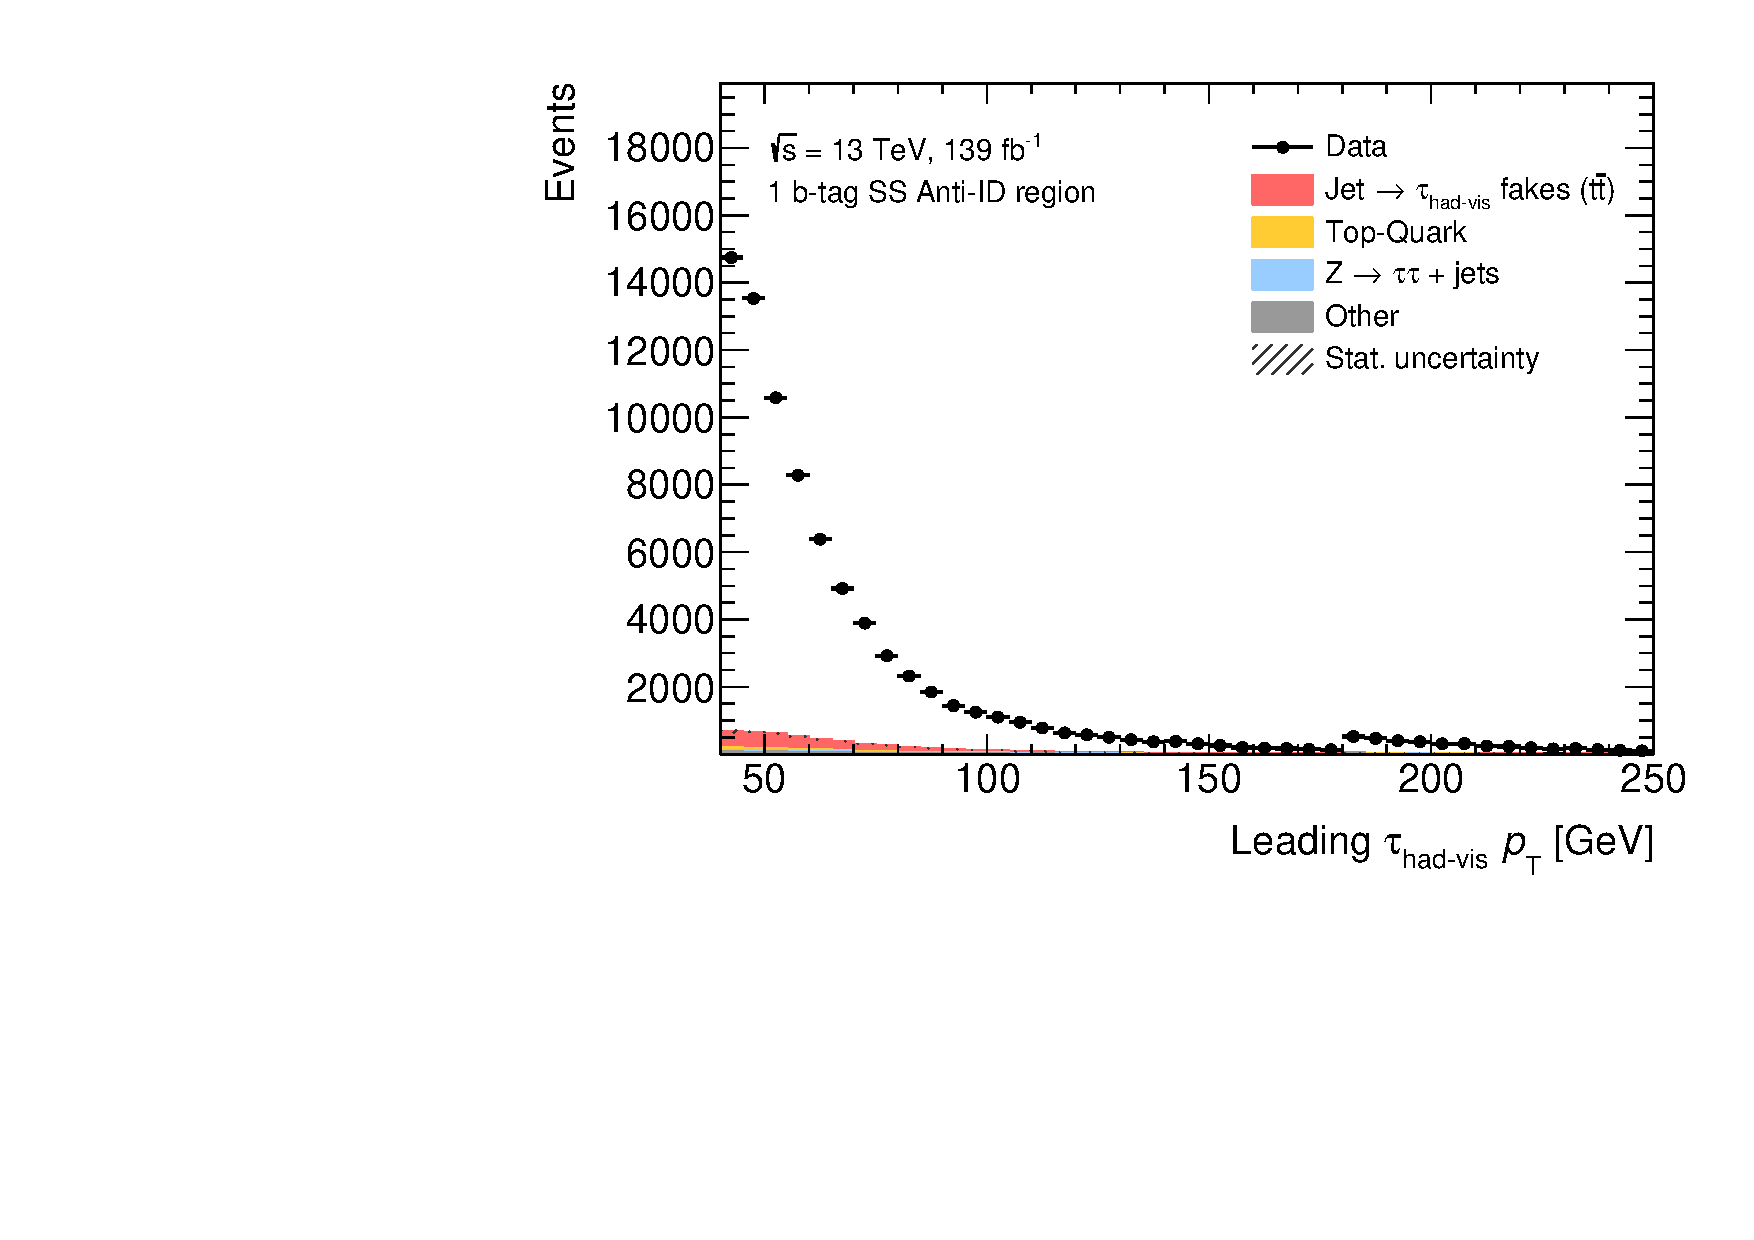
\includegraphics[width=\textwidth]{fakefactors/region_plots/tau0pt_1tag_ss_antiid}
    \subcaption{1 $b$-tag SS Anti-ID region}
  \end{subfigure}
  \begin{subfigure}{0.49\textwidth}
    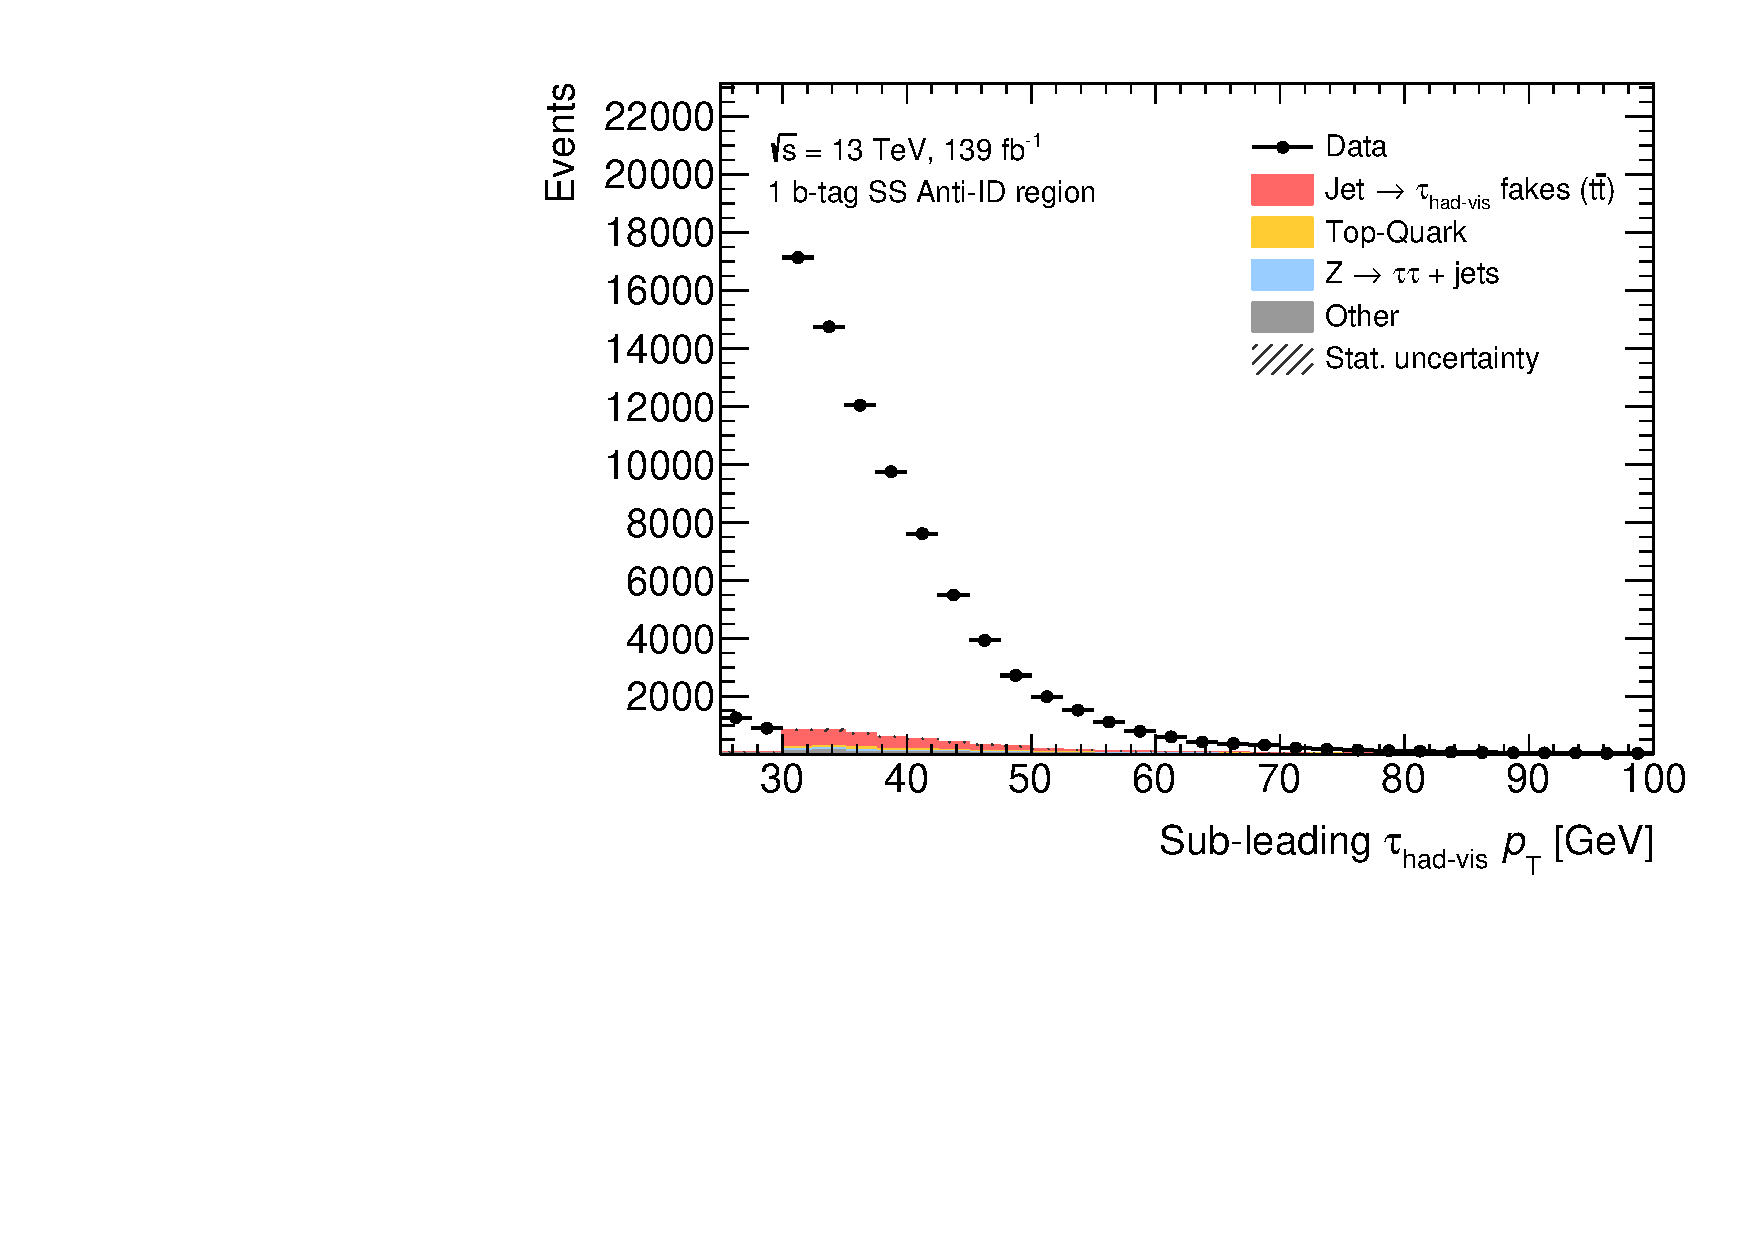
\includegraphics[width=\textwidth]{fakefactors/region_plots/tau1pt_1tag_ss_antiid}
    \subcaption{1 $b$-tag SS Anti-ID region}
  \end{subfigure}

  \caption[Distribution of the leading and sub-leading \tauhadvis \pT for
  observed data and non-multi-jet backgrounds in regions used for the FF
  measurement.]{Distribution of the leading and sub-leading \tauhadvis \pT for
    observed data and non-multi-jet backgrounds in regions used for the FF
    measurement. The 1 $b$-tag SS ID region is shown in (a,b) and the 1 $b$-tag
    SS Anti-ID region in (c,d). Coloured histograms depict the contributions of
    non-multi-jet processes that are subtracted when estimating the FFs. The
    difference between the observed data and the non-multi-jet background
    estimate is attributed to the missing multi-jet background.}%
  \label{fig:mjfakes_1tag_ss_plots}
\end{figure}

A schematic illustration of the approach is given
in~\Cref{fig:fakefactor_regions}. FFs measured in the 1 $b$-tag SS regions
($\text{FF}_\text{SS}^\text{1-tag}$) are applied to events in the 2 $b$-tag OS
Anti-ID region after subtraction of non-multi-jet contributions to obtain an
estimate of the multi-jet background in the SR. Multiplicative transfer factors
($\text{TF}_{1 \ra 2\,b\text{-tag}}$) are applied to
$\text{FF}_\text{SS}^\text{1-tag}$ when used in 2 $b$-tag regions, accounting
for possible differences between FFs measured in 1 and 2 $b$-tag regions and the
uncertainties associated with this extrapolation. The 1 $b$-tag OS ID region
serves as a validation region (VR) to check the agreement of the background
prediction with the observed data. Any non-closure observed in this region
indicates either a violation of the assumptions of the FF method, or
dependencies that are not captured by the parameterisation of the FFs.

\begin{figure}[htbp]
  \centering

  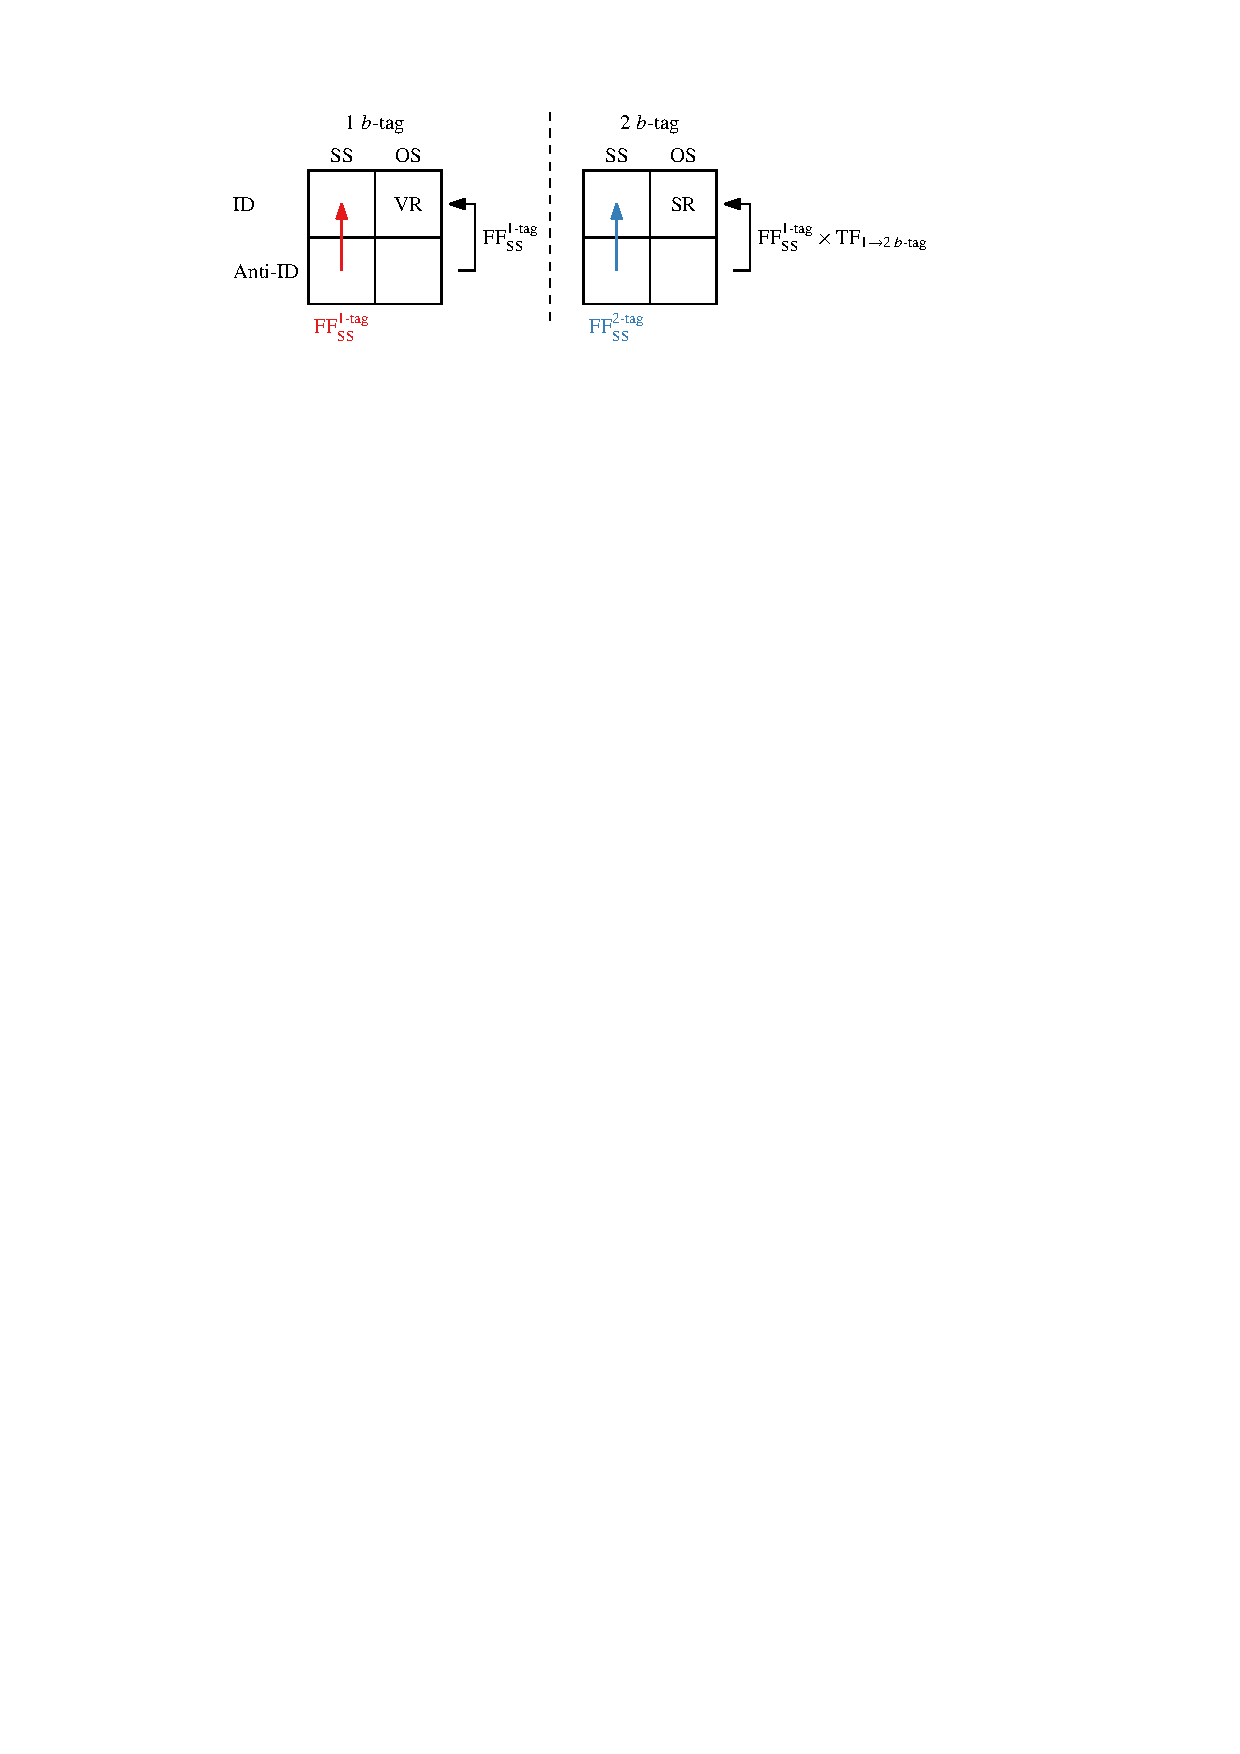
\includegraphics[scale=1]{fakefactors/regions}

  \caption[Schematic description of the FF method used to estimate the multi-jet
  background in the SR of the \hadhad channel.]{Schematic description of the FF
    method used to estimate the multi-jet background in the SR of the \hadhad
    channel. The squares represent the multi-jet events
    ($N_\text{multi-jet} = N_\text{data} - N_\text{non-multi-jet}$) in a
    particular region. The red / blue arrows correspond to FFs calculated as the
    ratio of multi-jet events in ID and Anti-ID regions. Black arrows correspond
    to the application of FFs in the OS Anti-ID region to obtain the multi-jet
    template in the OS ID region.}
  \label{fig:fakefactor_regions}
\end{figure}

% % verify the independence of the observables related to \tauid and
% % electric charge of the \tauhadvis pair.
% This approach is equivalent to a comparison of fake factors measured
% in the OS and SS regions\footnote{\Cref{tab:mjfakes_yields_1tag} can
%   be used to calculate inclusive fake factors in the OS and SS
%   regions, yielding
%   $\text{FF}_\text{SS}^\text{1-tag} \approx
%   \text{FF}_\text{OS}^\text{1-tag} \approx 0.18$, which is a
%   sufficient condition for statistical independence of the fake factor
%   observables at the level of the inclusive selection.}, which have to
% agree under the assumptions of the method.\todo{Needs some work...}


\subsubsection{Binning of the Fake Factor Measurement}

% Binning in years / trigger
The FF measurement is performed separately for events selected by STTs and DTTs
to account for the differences in selection applied by these triggers. STTs
require one \tauhadvis candidate with high transverse momentum passing the HLT
\tauid, while DTTs require two \tauhadvis candidates both passing HLT \tauid and
significantly lower \pT~thresholds. In addition, the changes in
\tauhadvis-triggers during Run~2 of the LHC are accounted for by performing the
FF measurement separately for three major data-taking periods:~2015--2016, 2017,
and 2018.

% Reason for binning
%
% The categorisation of the FFs by trigger that selected the event is further
% motivated by the differences between both trigger categories. STTs require one
% \tauhadvis candidate with high transverse momentum that is identified at the
% HLT without any selections applied to the other candidate. In contrast, DTTs
% require two \tauhadvis to be identified at the HLT with similar transverse
% momentum thresholds applied to both. This allows \tauhadvis candidates in the
% DTT to be treated equally once \pT~threshold effects are accounted for.

Dependencies of FFs on properties of reconstructed \tauhadvis candidates are
accounted for by further categorisation based on properties of the
(anti-)\tauhadvis that distinguishes the ID from the Anti-ID regions. The FF
measurement is performed separately for 1- and 3-prong \tauhadvis candidates for
both trigger categories. For events selected by DTTs, the FFs are additionally
measured in bins of the \tauhadvis candidate~\pT and separately for candidates
in the barrel ($|\eta| < 1.37$) and end-cap ($|\eta| \geq 1.52$) regions of the
detector. Few multi-jet events are selected by STTs due to the large
\pT~thresholds on \tauhadvis candidates, preventing a fine binning of the FF
measurement. In this case, FFs are measured separately for cases where the
anti-\tauhadvis is leading in \pT and sub-leading in \pT. This accounts for the
\tauid applied at the HLT and the large difference in transverse momentum
between the leading and sub-leading \tauhadvis candidate.

% In contrast, few multi-jet events are selected by STTs due to high \pT
% thresholds on \tauhadvis preventing fine subdivision of the FF
% measurement. Therefore, FFs for events selected by STTs are measured
% separately for cases where the anti-\tauhadvis is leading and sub-leading in
% \pT. This accounts for the \tauid applied at the HLT and the transverse
% momentum differences between the leading and sub-leading
% \tauhadvis~candidates.

\subsubsection{Measurement of Fake Factors for Events Selected by DTTs}

{% Group for extra definitions
  \newcommand*{\ffargs}{\ensuremath{( \myvec{x}_{\tau} )}\xspace}

  \newcommand*{\NmjID}[2]{\ensuremath{N_\text{multi-jet}^{\text{#1, loose }\tau_{#2}}}\xspace}
  \newcommand*{\NmjIDIncl}[1]{\ensuremath{N_\text{multi-jet}^{\text{#1, ID}}}\xspace}

  \newcommand*{\NmjAntiIDIncl}[1]{\ensuremath{N_\text{multi-jet}^{\text{#1, Anti-ID}}}\xspace}
  \newcommand*{\NmjAntiID}[2]{\ensuremath{N_\text{multi-jet}^{\text{#1, anti-}\tau_{#2}}}\xspace}

  The Anti-ID region can be split into two subregions: one where the
  anti-\tauhadvis is the leading and one where it is the sub-leading \tauhadvis
  candidate. Provided the conditions for the FF method are fulfilled, both
  regions can be used to obtain separate estimates of the multi-jet background
  in the OS ID region. The notation used to describe the FF measurement is
  introduced in the following:
  \begin{description}[style=standard]
  \item[$\tau_0$ ($\tau_1$)] The \tauhadvis candidate leading (sub-leading) in \pT.

  \item[$\myvec{x}_\tau$] A vector of categorical observables of the
    reconstructed \tauhadvis candidate that specifies the bin of the FF
    measurement.
    % For the DTT category, these correspond to the bin in \Ntracks, \pT, and
    % $\eta$.

  \item[$\NmjID{SS(OS)}{i}\ffargs$] The estimated number of multi-jet events in
    the SS (OS) ID region where~$\tau_i$ falls into the bin specified
    by~$\myvec{x}_\tau$.

  \item[$\NmjAntiID{SS(OS)}{i}\ffargs$] The estimated number of multi-jet events
    in the SS (OS) Anti-ID region where $\tau_i$ is the anti-\tauhadvis and
    falls into the bin specified by~$\myvec{x}_\tau$.
  \end{description}
  With these definitions, two sets of FFs can be defined as
  \begin{align*}
    \FF_{i}\ffargs &= \frac{\NmjID{SS}{i} \ffargs}{\NmjAntiID{SS}{i}\ffargs}
                     \quad \text{for} \quad i = 0, 1 \,\text{,}
  \end{align*}
  where $\FF_{i}$ is the FF relating the ID region with the partition of the
  Anti-ID region where $\tau_i$ is the anti-\tauhadvis. These can be used to
  obtain two multi-jet estimates in the OS region given by
  \begin{align*}
    \NmjID{OS}{i}\ffargs = \FF_{i}\ffargs \cdot \NmjAntiID{OS}{i}\ffargs
    \quad \text{for} \quad i = 0, 1 \,\text{.}
  \end{align*}
  The average of both estimates also yields an estimate of the multi-jet
  background. The process of averaging both multi-jet estimates can be expressed
  by an alternative set of FFs that do not distinguish in whether the
  anti-\tauhadvis is the leading or sub-leading \tauhadvis candidate, thus
  acting on the entirety of the Anti-ID region instead of a subregion
  thereof. This inclusive FF is given by
  \begin{align*}
    \FF_\text{incl.}\ffargs = \frac{1}{2} \left[ f_0\ffargs \cdot \FF_0\ffargs
    + f_1\ffargs \cdot \FF_1\ffargs \right] \,\text{,}
  \end{align*}
  with $f_i\ffargs$ being the fraction of anti-\tauhadvis in the bin given by
  $\myvec{x}_\tau$ that are leading ($i = 0$) or sub-leading ($i = 1$) in \pT,
  formally given by
  \begin{align*}
    f_i\ffargs = \frac{\NmjAntiID{SS}{i}\ffargs}
                      {\NmjAntiID{SS}{0}\ffargs + \NmjAntiID{SS}{1}\ffargs} \,\text{.}
  \end{align*}
  The inclusive FF can be measured directly using the following relationship
  \begin{align}
    \FF_\text{incl.}\ffargs
    = \frac{1}{2} \frac{ \NmjID{SS}{0}\ffargs + \NmjID{SS}{1}\ffargs }
                       { \NmjAntiID{SS}{0}\ffargs + \NmjAntiID{SS}{1}\ffargs } \,\text{,}
    \label{eq:inclusive_fake_factor}
  \end{align}
  which can be applied to events in the inclusive Anti-ID region to obtain the
  multi-jet estimate in the ID region.

  % and the multi-jet estimate in the OS region obtained by\todo{Should there be a $\sum_{x_\tau}$ here?}
  % \begin{align*}
  %   \NmjIDIncl{OS}\ffargs = \FF_\text{incl.}\ffargs \cdot \NmjAntiIDIncl{OS}\ffargs \,\text{,}
  % \end{align*}
  % where $\NmjAntiIDIncl{OS}\ffargs$ is the number of multi-jet events
  % in the inclusive OS Anti-ID region with anti-\tauhadvis in the bin
  % given by~$\myvec{x}_\tau$.

  % Prior the agreement of the background estimates obtained with FF0
  % and FF1 were confirmed.

  The motivation of using the approach of defining inclusive FFs is twofold:
  First, it allows using all events in the Anti-ID region, independent of
  whether the anti-\tauhadvis is leading or sub-leading in \pT, thus improving
  the statistical precision of the background estimate. Second, the FFs can be
  parameterised in properties of the anti-\tauhadvis directly, allowing to
  target the key differences between the ID and Anti-ID regions. This represents
  a change with respect to the previous publication in
  Ref.~\cite{HIGG-2016-16-witherratum} in which FFs were parameterised in the
  properties of both \tauhadvis candidates simultaneously. The high
  dimensionality of the FF parameterisation was a limitation in the previous
  measurement.}

% The inclusive FFs for events selected by DTTs are measured according
% to~\Cref{eq:inclusive_fake_factor} and parameterised in \tauhadvis decay mode,
% transverse momentum, pseudorapidity, and the period of data-taking. The number
% of multi-jet events is obtained by subtracting the expected number of
% non-multi-jet events estimated using simulation from the number of observed
% events in data.

The result of the FF measurement for DTTs is summarised
in~\Cref{fig:mjfakes_fake_factors}. Qualitatively, the behaviour of the FFs with
respect to \tauhadvis candidate properties is the same between data-taking
periods. Minor differences can be observed when comparing FFs between years. No
attempt was made to combine the measurements as the statistical precision of the
FF measurement is not a limiting factor in the analysis.

\begin{figure}[htbp]
  \centering

  \begin{subfigure}{0.495\textwidth}
    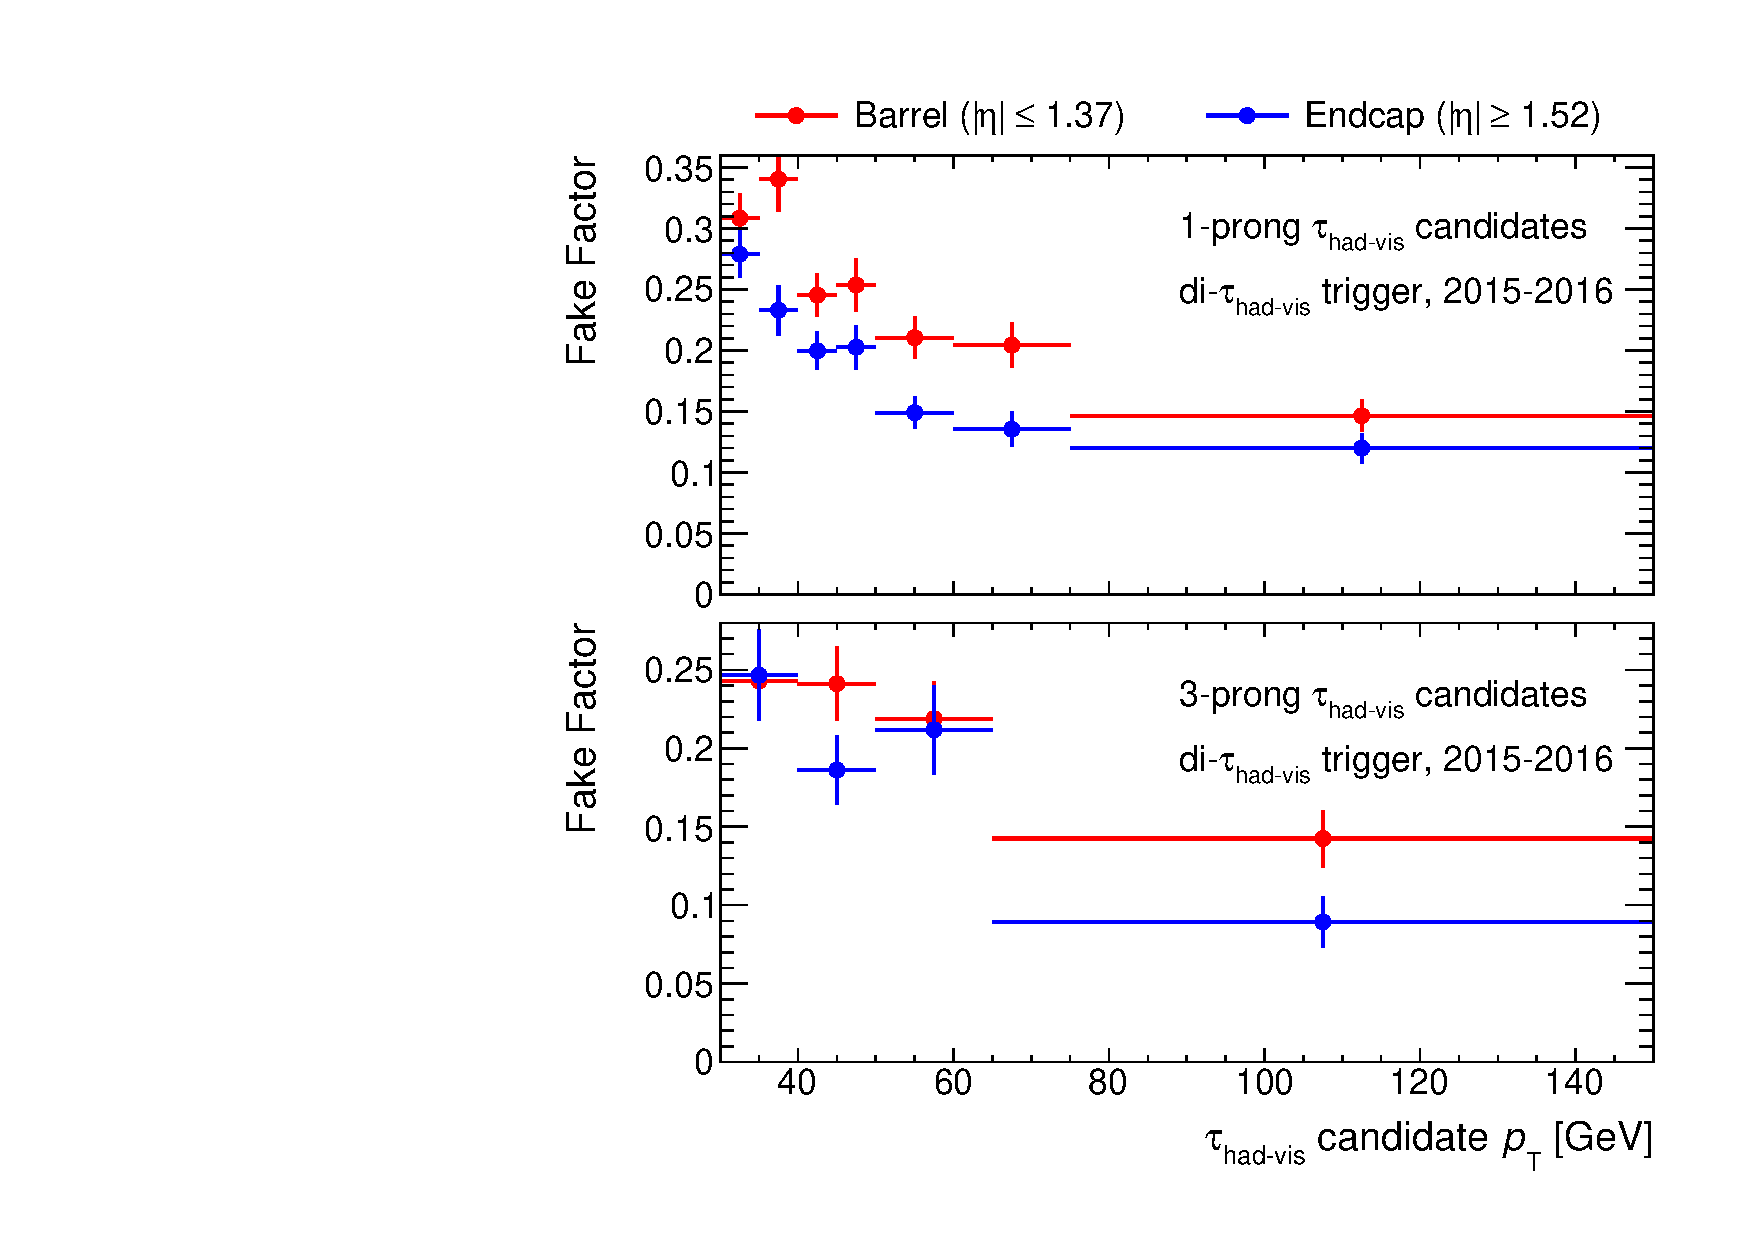
\includegraphics[width=\textwidth]{fakefactors/fake_factors_dtt_1516}
    \subcaption{2015--2016 data-taking period}
  \end{subfigure}
  \begin{subfigure}{0.495\textwidth}
    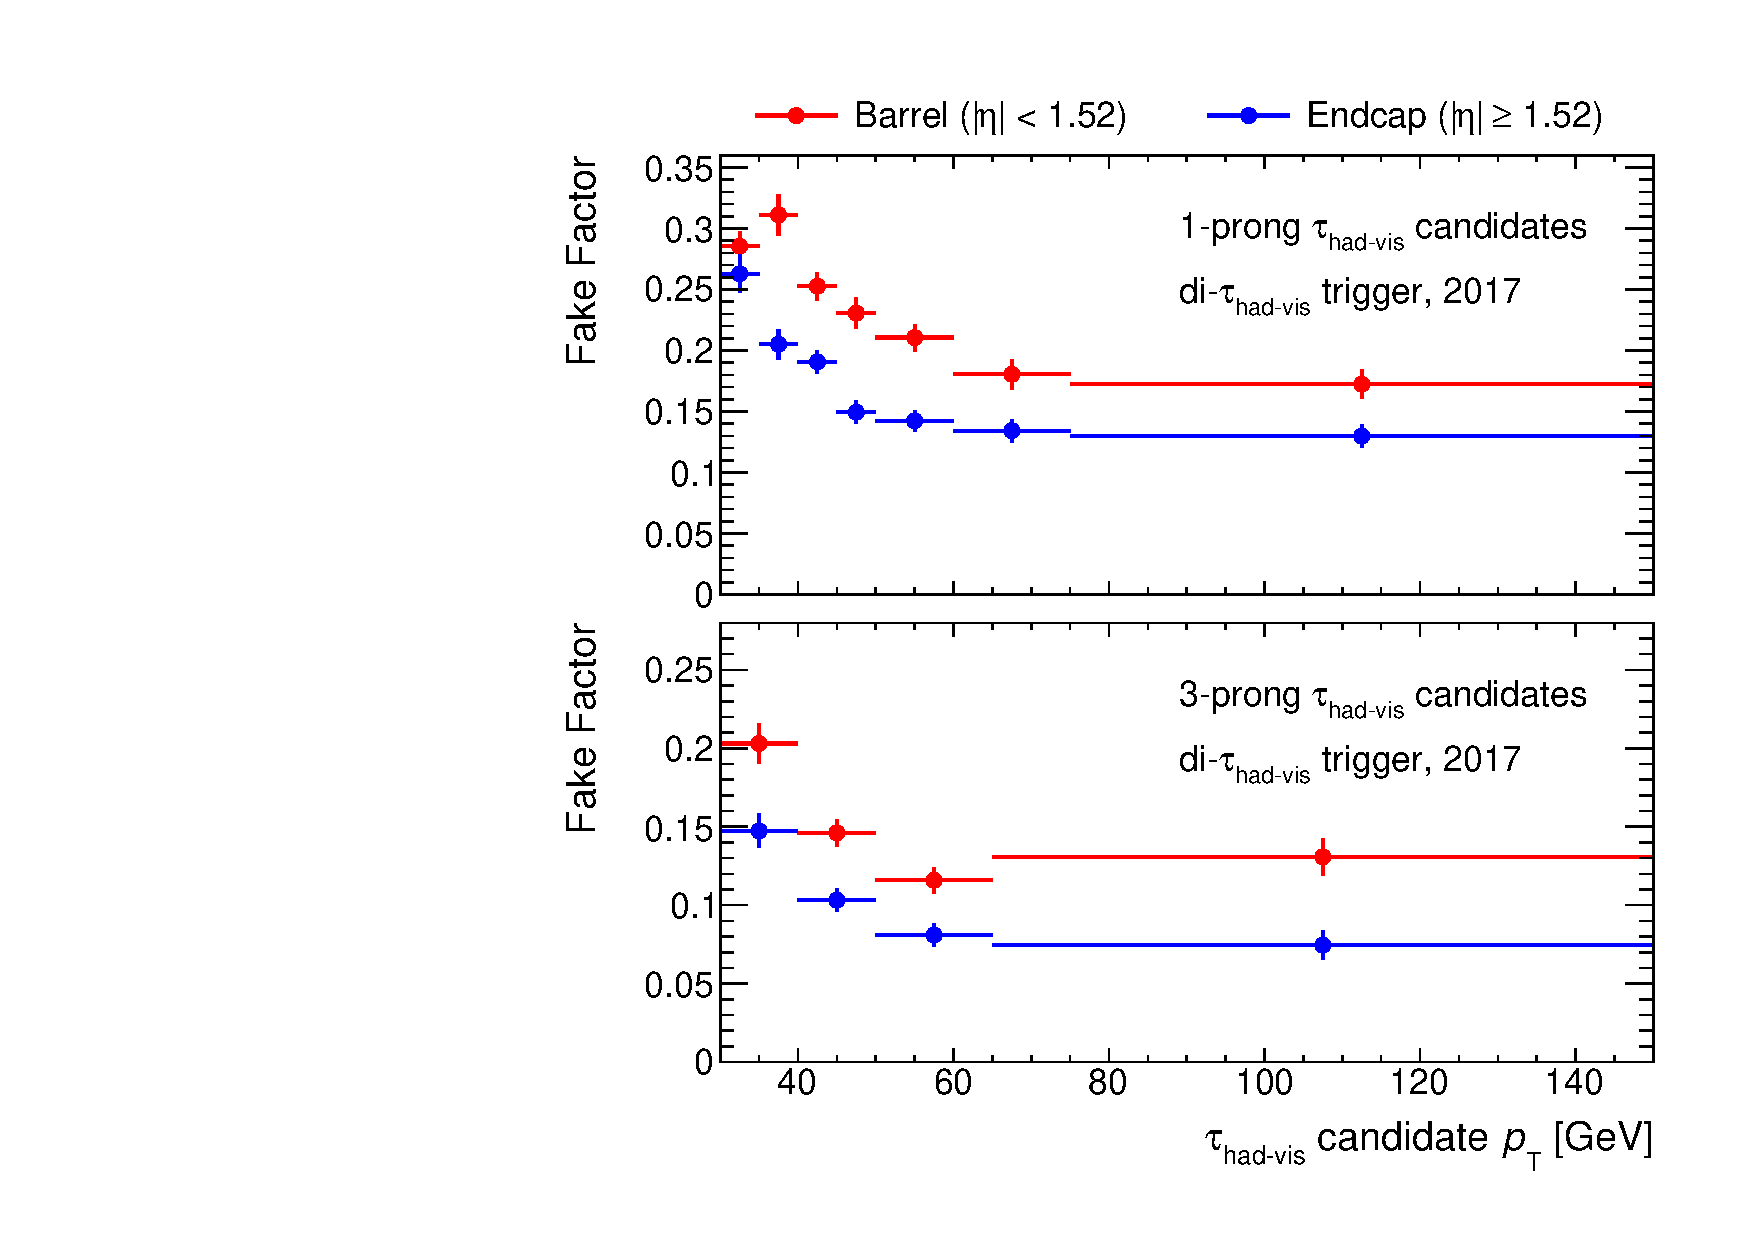
\includegraphics[width=\textwidth]{fakefactors/fake_factors_dtt_17}
    \subcaption{2017 data-taking period}
  \end{subfigure}

  \begin{subfigure}{0.495\textwidth}
    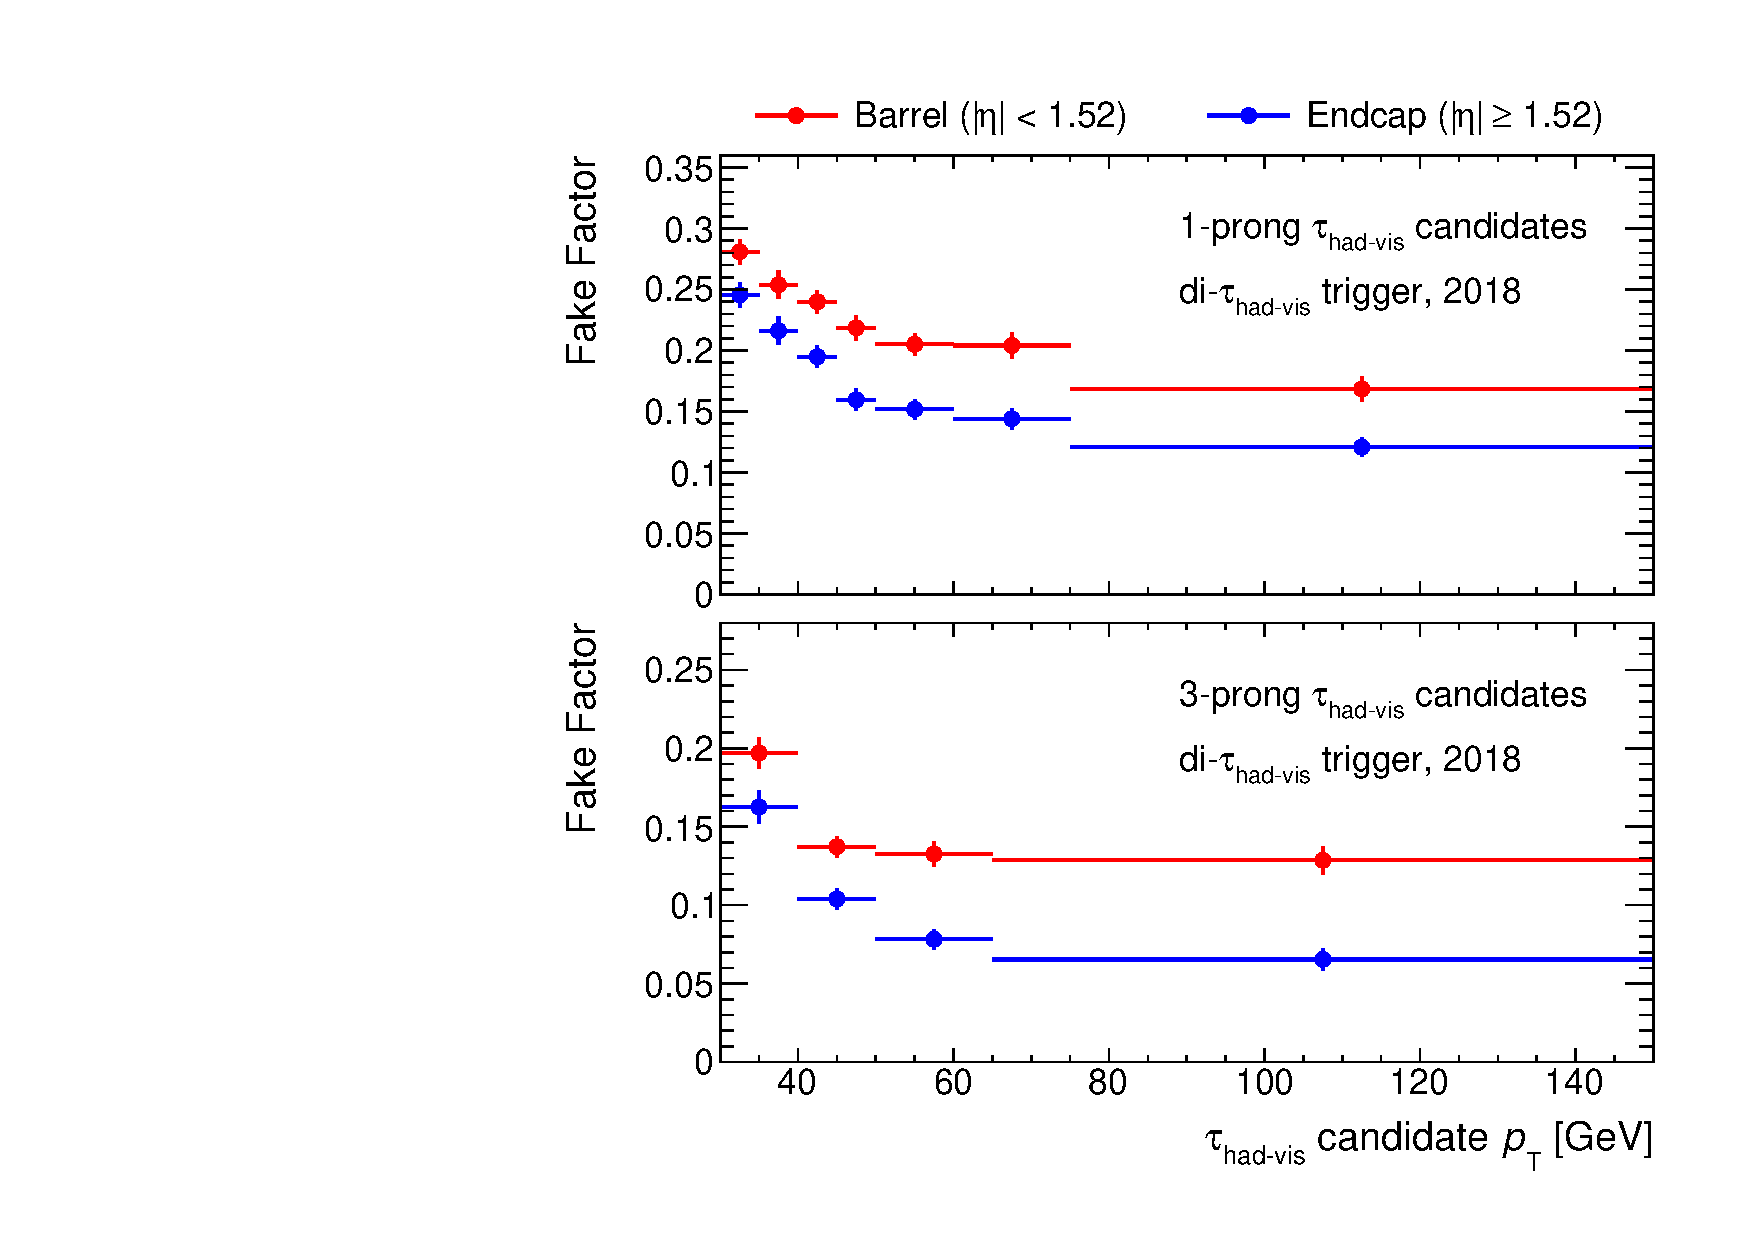
\includegraphics[width=\textwidth]{fakefactors/fake_factors_dtt_18}
    \subcaption{2018 data-taking period}
  \end{subfigure}

  \caption[Fake factors for DTT events.]{DTT FFs measured in the 1 $b$-tag SS
    region. The measurement is performed separately for the three major
    data-taking periods (a-c), 1- and 3-prong \tauhadvis candidates (upper/lower
    panels), and for \tauhadvis in the barrel (red) and end-cap (blue) regions
    of the ATLAS detector. Events with (anti-)\tauhadvis $\pT > \SI{150}{\GeV}$
    are included in the last FF bin. Only statistical uncertainties are
    shown. Systematic uncertainties originating from the non-multi-jet
    subtraction are assumed to be negligible due to the small size of the
    subtraction in the 1 $b$-tag SS region.}%
  \label{fig:mjfakes_fake_factors}
\end{figure}


\subsubsection{Measurement of Fake Factors for Events Selected by STTs}

The measurement of FFs for events selected by STTs can proceed
using~\Cref{eq:inclusive_fake_factor}. The measured STT FFs are shown
in~\Cref{fig:mjfakes_stt_ffs} for the three major data-taking periods. Each
period is divided into four categories depending on $N_{\text{tracks}}$ and
whether the anti-\tauhadvis is leading ($\tau_0$) or sub-leading ($\tau_1$) in
\pT.

% The measurement of FFs for events selected by STTs proceeds differently from
% the DTT case. Due to the selections applied at the HLT and the usually large
% difference in \pT between both \tauhadvis candidates, the STT FFs are measured
% separately for the leading and sub-leading \tauhadvis
% candidates. Additionally, the high \pT thresholds on \tauhadvis at
% trigger-level provide large rejection of most SM processes, limiting the
% number of events entering the CRs for the FF measurement, thus preventing a
% differential FF measurement in \tauhadvis \pT and $\eta$.

% The approach of averaging the background estimates obtained from the two
% partitions of the Anti-ID region remains valid for STTs,
% including~\Cref{eq:inclusive_fake_factor} which can be used to calculate the
% FFs. The main difference between the the STT and DTT FF measurement is the
% replacement of the variables specifying the \pT and $\eta$ bin in
% $\myvec{x}_\tau$ with an indicator variable specifying whether the
% anti-\tauhadvis is leading or sub-leading in \pT.

% First, at the HLT \tauhadvis identification is only applied to one of the
% \tauhadvis candidates, preventing an inclusive treatment of both \tauhadvis
% candidates. Second, the high \pT thresholds on \tauhadvis at trigger-level has
% high rejection of most SM processes, limiting the number of events entering
% the control regions for the fake factor measurement. As a result, the fake
% factors for singe-\tauhadvis triggers cannot be measured differentially in
% \tauhadvis \pT and $\eta$.

\begin{figure}[htbp]
  \centering

  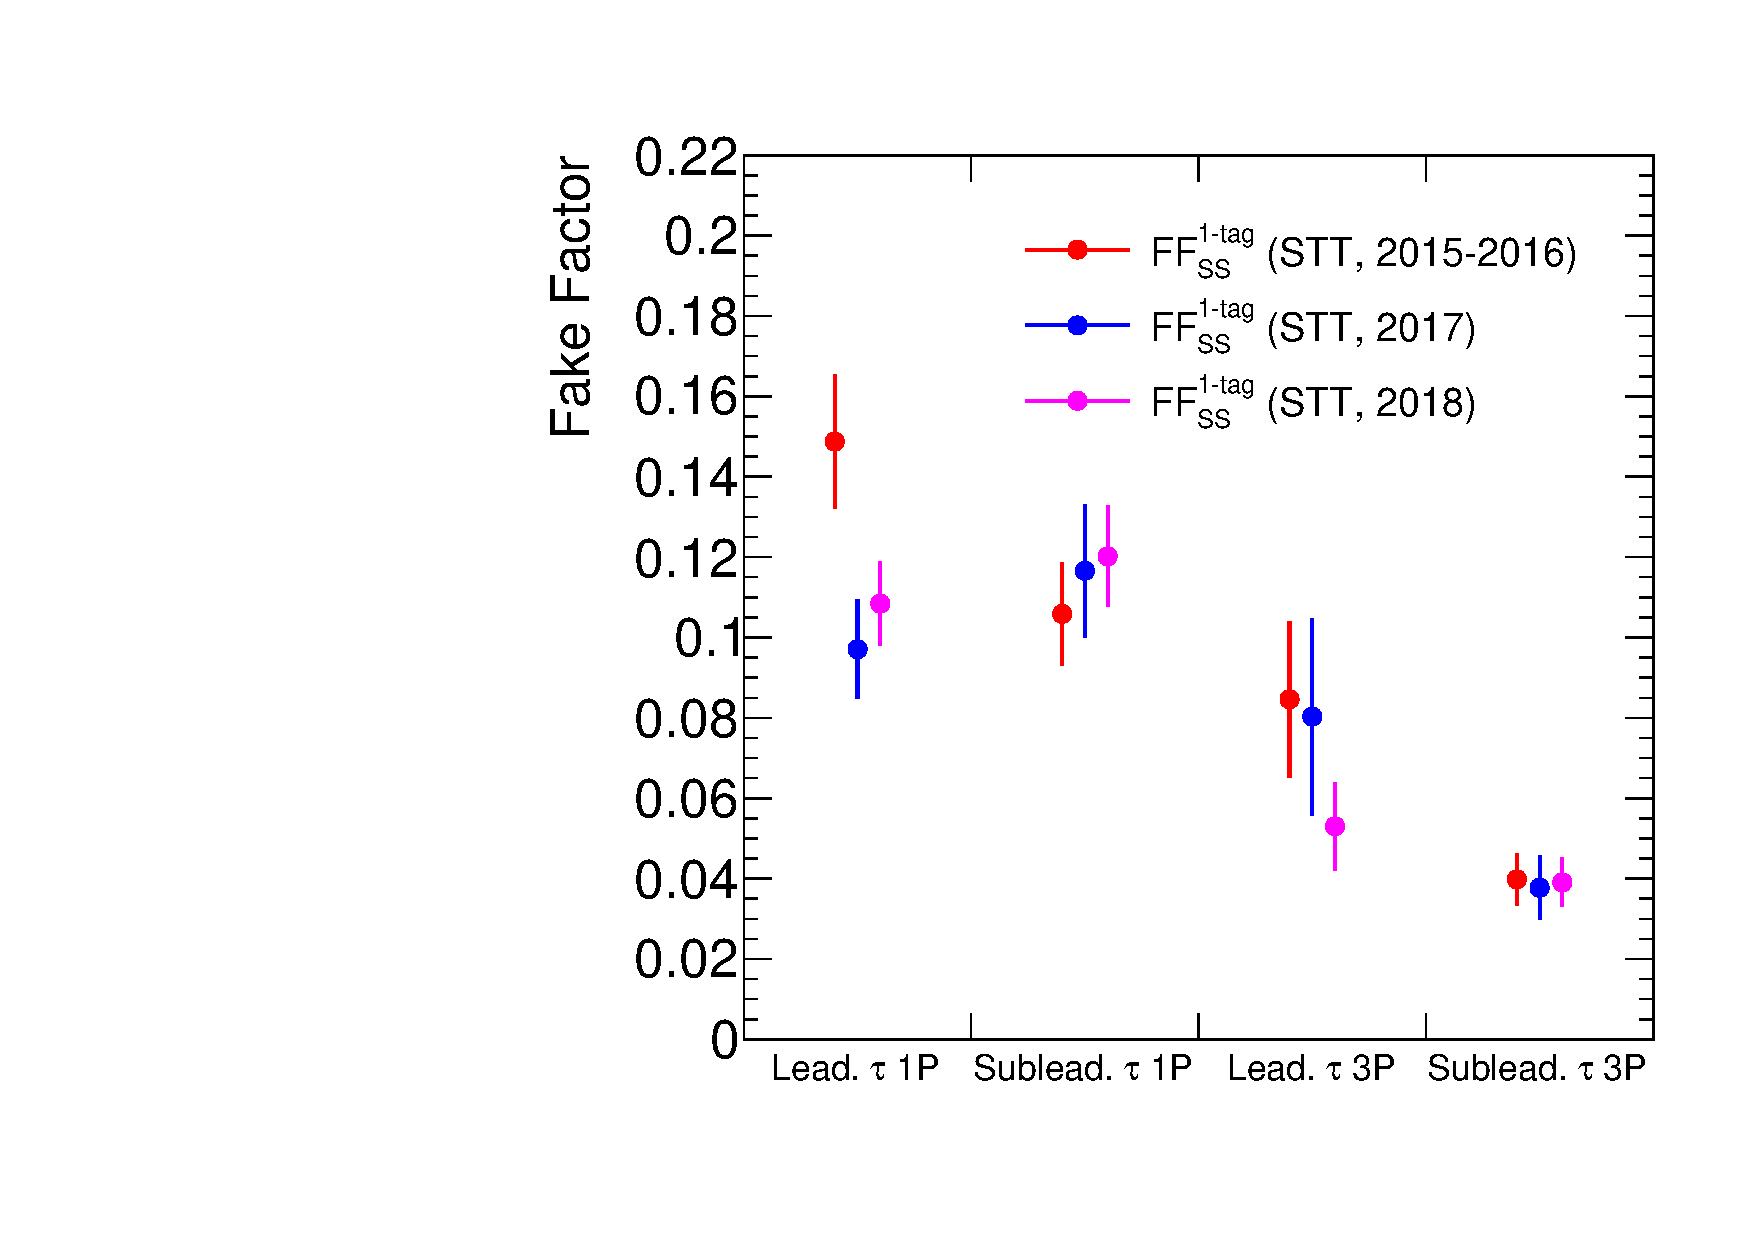
\includegraphics[width=0.495\textwidth]{fakefactors/fake_factors_stt}

  \caption[Fake factors for STT events.]{STT FFs measured in the
    1~$b$-tag~SS~region separately for the three major data-taking periods. The
    measurement is performed in bins of the \tauhadvis candidate~\Ntracks (1-
    and 3-prong) and separately for cases where the anti-\tauhadvis is leading
    ($\tau_0$) and sub-leading in \pT ($\tau_1$). Only statistical uncertainties
    are shown.}%
  \label{fig:mjfakes_stt_ffs}
\end{figure}

\subsubsection{Validation of the Multi-jet Estimate in the 1 $b$-tag OS Region}

An independent validation of the background estimate is performed in the 1
$b$-tag OS ID region (cf.\ \Cref{fig:fakefactor_regions}). After the initial
event selection, this region has a multi-jet purity of about \SI{50}{\percent}
with the dominant non-multi-jet contributions originating from \Zjets and
\ttbar. A multi-jet validation region (VR) is defined by additionally requiring
events to fulfil
\begin{align*}
  \mMMC > \SI{110}{\GeV} \quad \text{and} \quad \mathcal{S} < 3 \,\text{,}
\end{align*}
where $\mathcal{S}$ is the object-based \pTmissAbs
significance~\cite{ATLAS-CONF-2018-038}. The \pTmissAbs significance measures
the statistical significance of a test comparing the hypothesis that the
reconstructed \pTmissAbs is compatible with zero within the expected measurement
errors to the alternative hypothesis of \pTmissAbs primarily originating from
undetected weakly interacting particles. The distributions of \mMMC and
$\mathcal{S}$ prior to the multi-jet VR selection are shown
in~\Cref{fig:fake_factor_OSVR_cutvars}. After the selection, the multi-jet
purity in the VR increases to \SI{75}{\percent} with a multi-jet selection
efficiency of about \SI{50}{\percent} with respect to the inclusive 1 $b$-tag OS
ID region.

% The distributions of the variables used to define the multi-jet VR are shown
% in~\Cref{fig:fake_factor_OSVR_cutvars} after pre-selection. The contribution
% of \Zjets is reduced by rejecting events with di-$\tauhad$ masses close to the
% \PZ boson mass.  Multi-jet events are expected to have little real \pTmissAbs,
% thus events with a significant \pTmissAbs measurement are rejected to reduce
% the \ttbar contribution in this region. The selection increases the multi-jet
% purity in the VR to \SI{75}{\percent} with a multi-jet selection efficiency of
% about \SI{50}{\percent} with respect to the pre-selection.

\begin{figure}[htbp]
  \centering

  \begin{subfigure}{0.44\textwidth}
    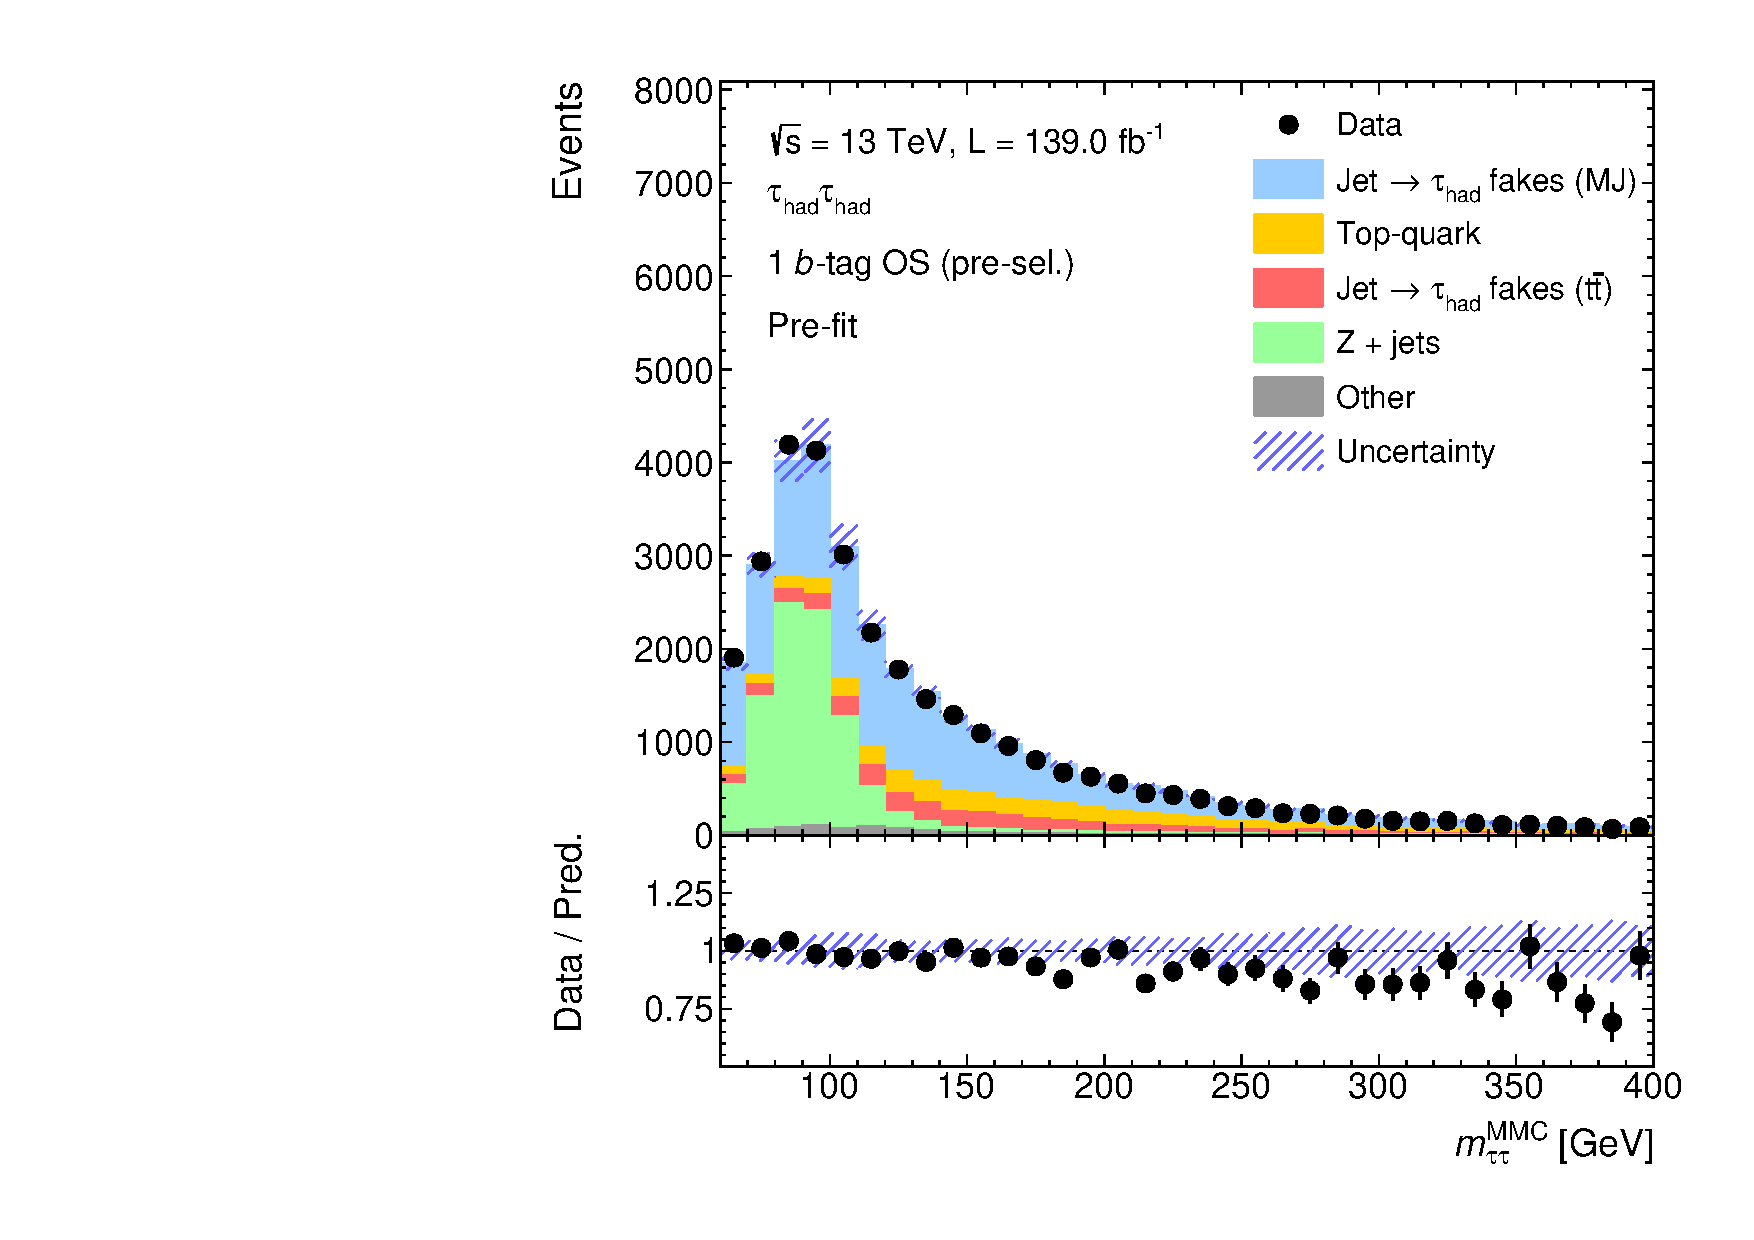
\includegraphics[width=\textwidth]{fakefactors/fake_os_vr/mMMC_presel}
    \subcaption{}
  \end{subfigure}\hspace*{0.04\textwidth}%
  \begin{subfigure}{0.44\textwidth}
    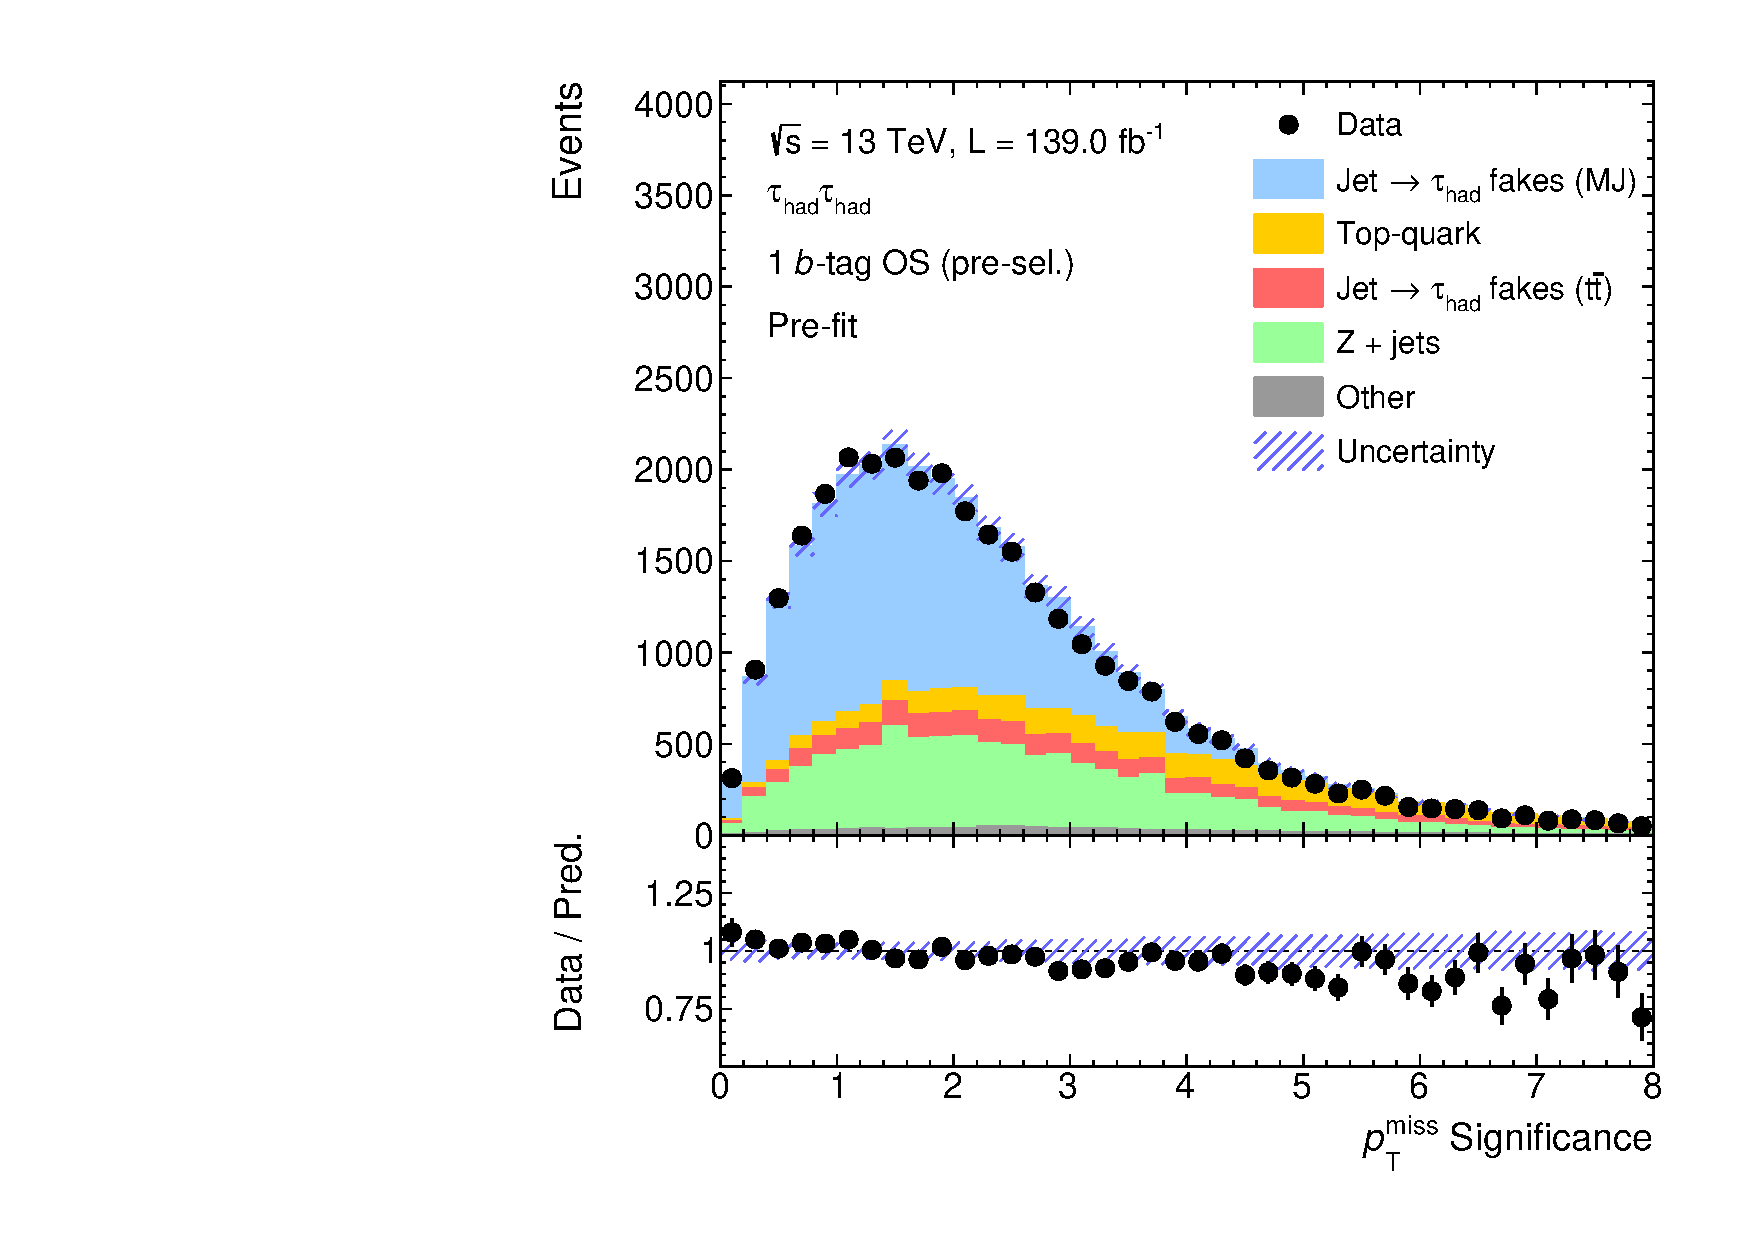
\includegraphics[width=\textwidth]{fakefactors/fake_os_vr/metSig_presel}
    \subcaption{}
  \end{subfigure}

  \caption[Distributions of \mMMC and the object-based \pTmissAbs significance
  in the 1 $b$-tag OS ID region.]{Distributions of the di-$\tau$ mass estimated
    with the MMC (a) and the object-based \pTmissAbs significance (b) in the 1
    $b$-tag OS ID region after the pre-selection. The estimate of the multi-jet
    background~(blue) is obtained using the FF method
    (cf.~\Cref{fig:fakefactor_regions}). Fake-\tauhadvis originating from
    \ttbar~(red) are estimated using simulation. The background prediction is
    shown pre-fit, including statistical and detector-related systematic
    uncertainties.}%
  \label{fig:fake_factor_OSVR_cutvars}
\end{figure}

The multi-jet background prediction in the VR is obtained by applying the
measured FFs to events in the OS Anti-ID region after subtracting non-multi-jet
contributions. The non-multi-jet backgrounds in the OS ID region are estimated
using simulation. The background prediction in the multi-jet VR is compared to
data in~\Cref{fig:fake_factor_OSVR_kinematics} for several observables of the
leading and sub-leading \tauhadvis candidate. Decent agreement between the
background prediction and data is observed in the VR for \tauhadvis-related
observables. A small mismodelling of the background is observed in the \pT
distribution of the sub-leading \tauhadvis candidate in the range of
\SIrange{60}{70}{\GeV} where the background appears to be overestimated by about
\SI{15}{\percent}. An uncertainty will be assigned to account for the
non-closure in the multi-jet VR.

\begin{figure}[htbp]
  \centering

  \begin{subfigure}{0.44\textwidth}
    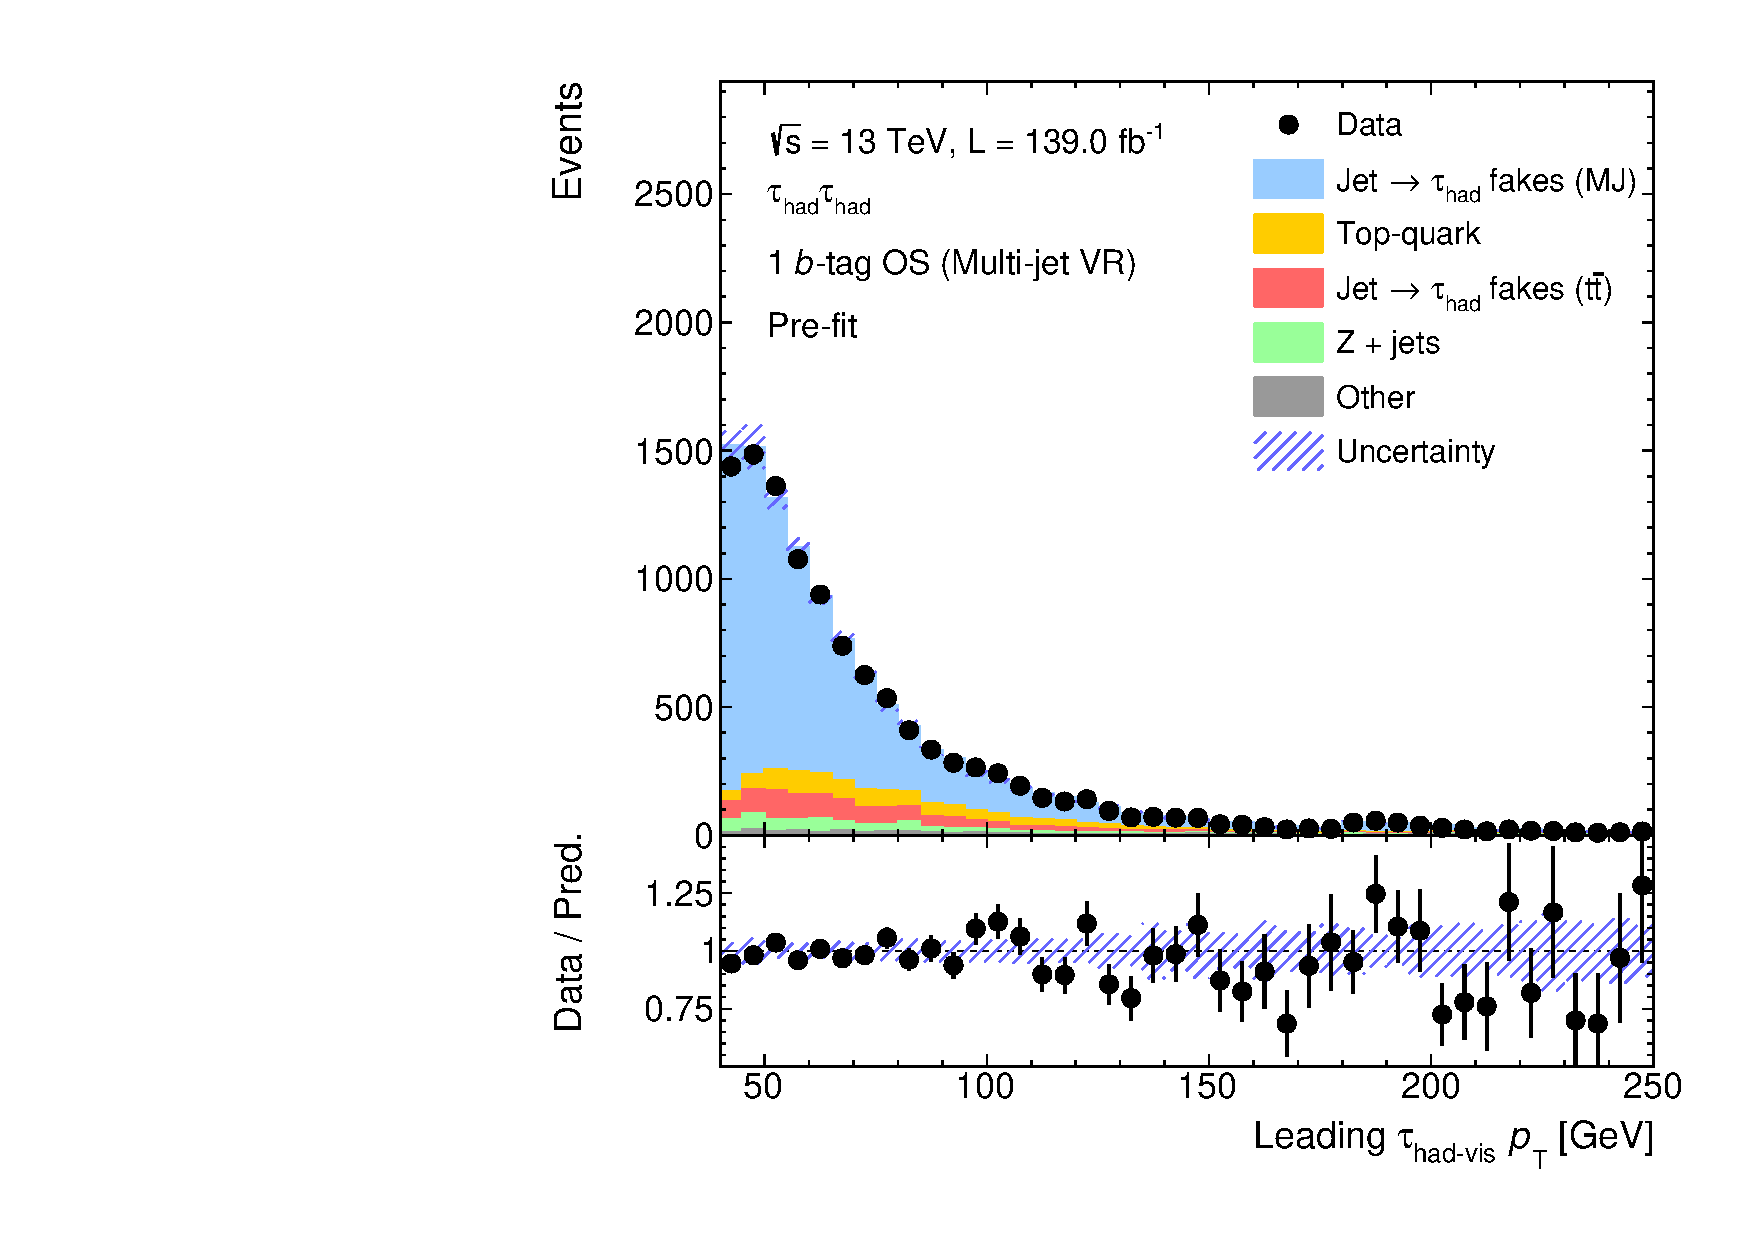
\includegraphics[width=\textwidth]{fakefactors/fake_os_vr/Tau0Pt_fakevr}
  \end{subfigure}\hspace*{0.04\textwidth}%
  \begin{subfigure}{0.44\textwidth}
    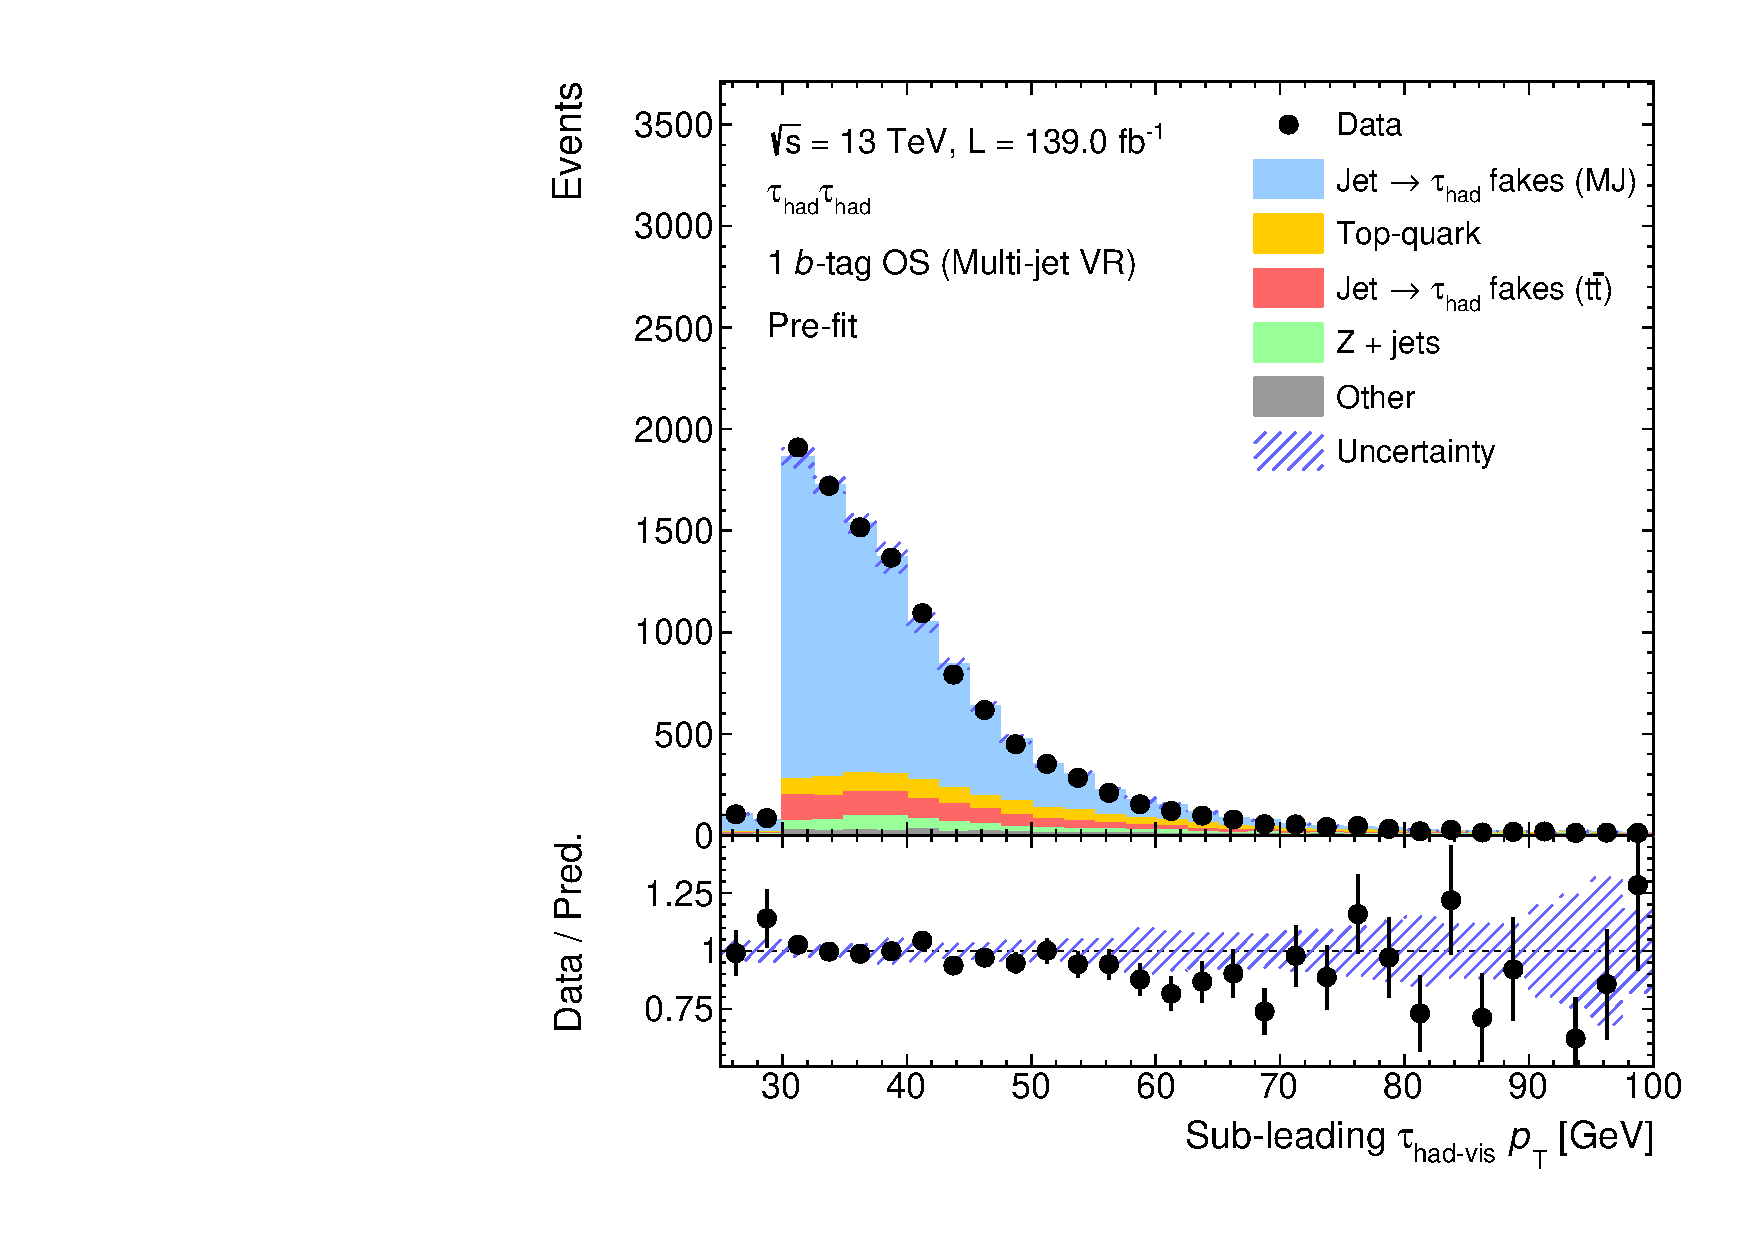
\includegraphics[width=\textwidth]{fakefactors/fake_os_vr/Tau1Pt_fakevr}
  \end{subfigure}

  \begin{subfigure}{0.44\textwidth}
    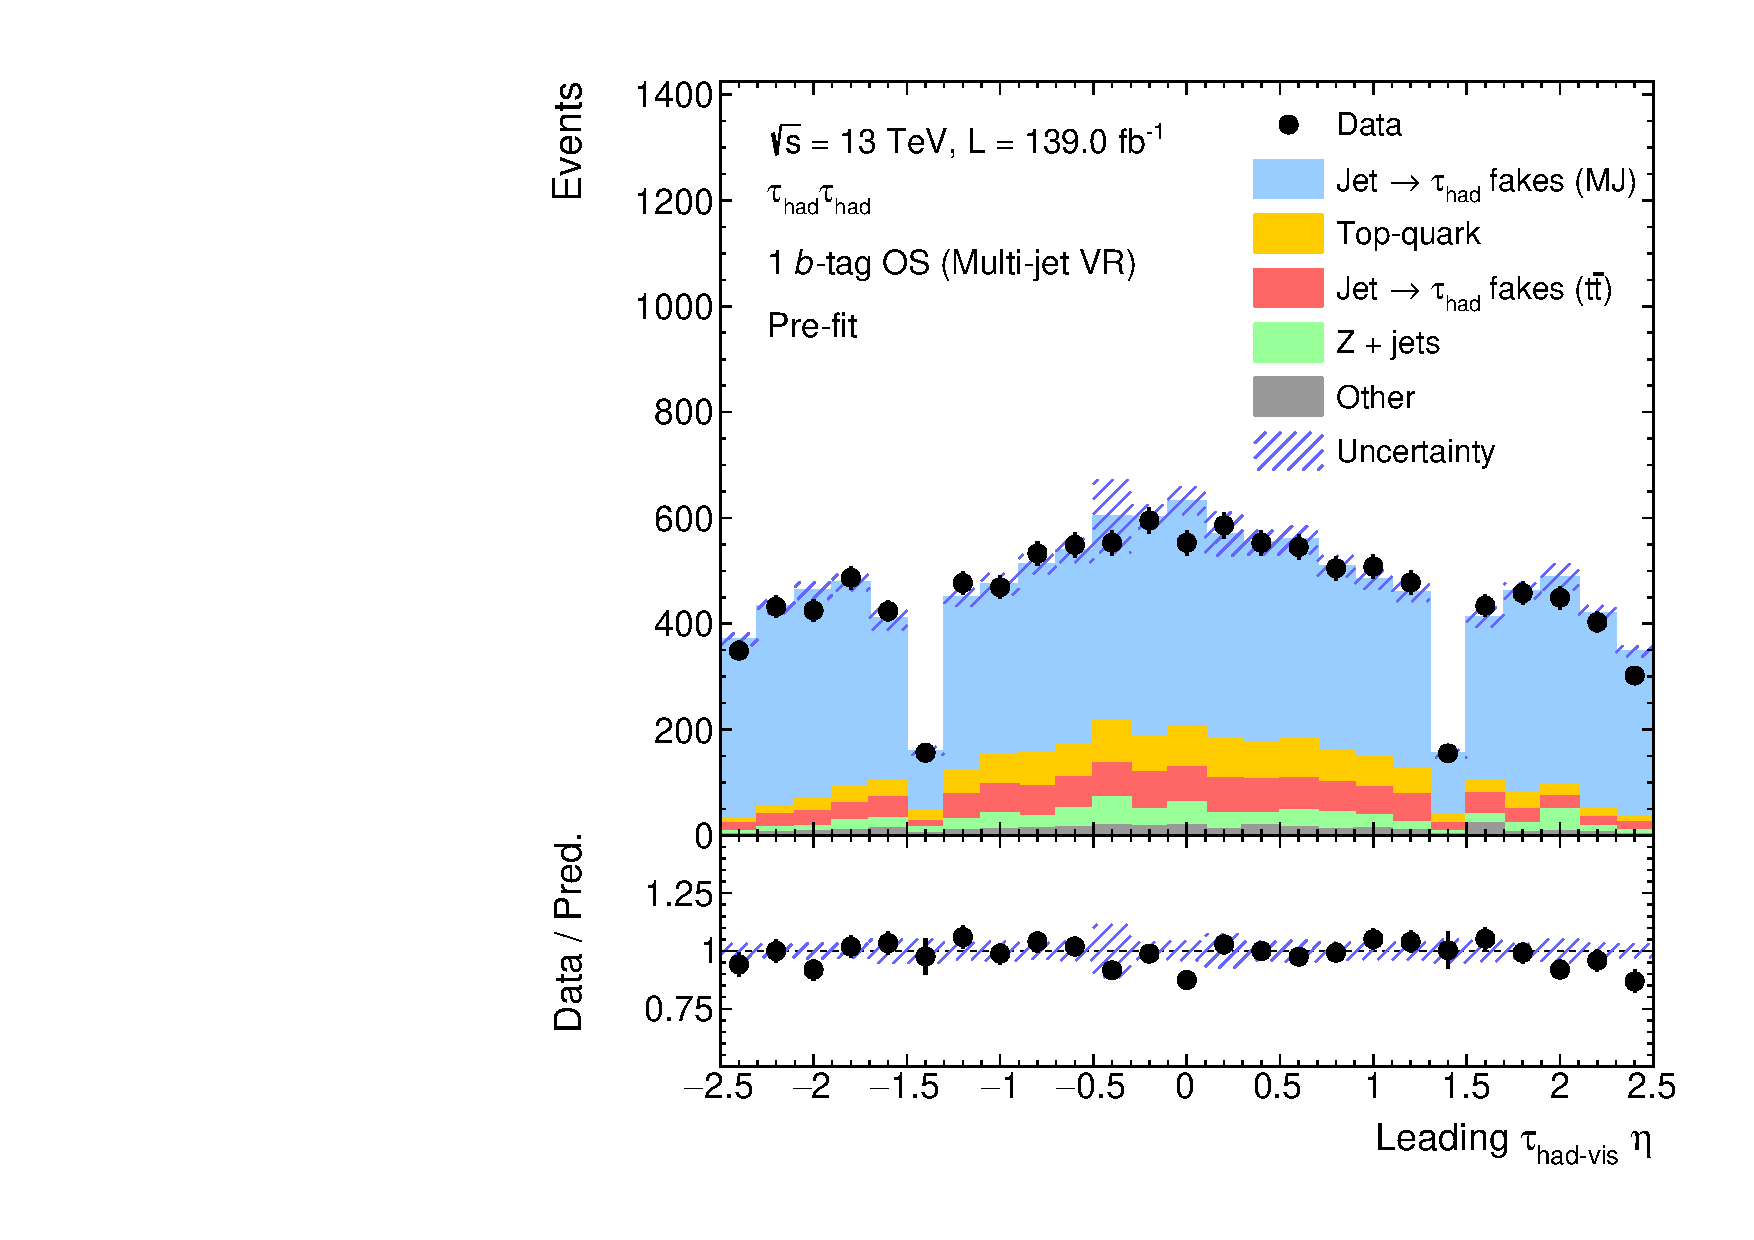
\includegraphics[width=\textwidth]{fakefactors/fake_os_vr/Tau0Eta_fakevr}
  \end{subfigure}\hspace*{0.04\textwidth}%
  \begin{subfigure}{0.44\textwidth}
    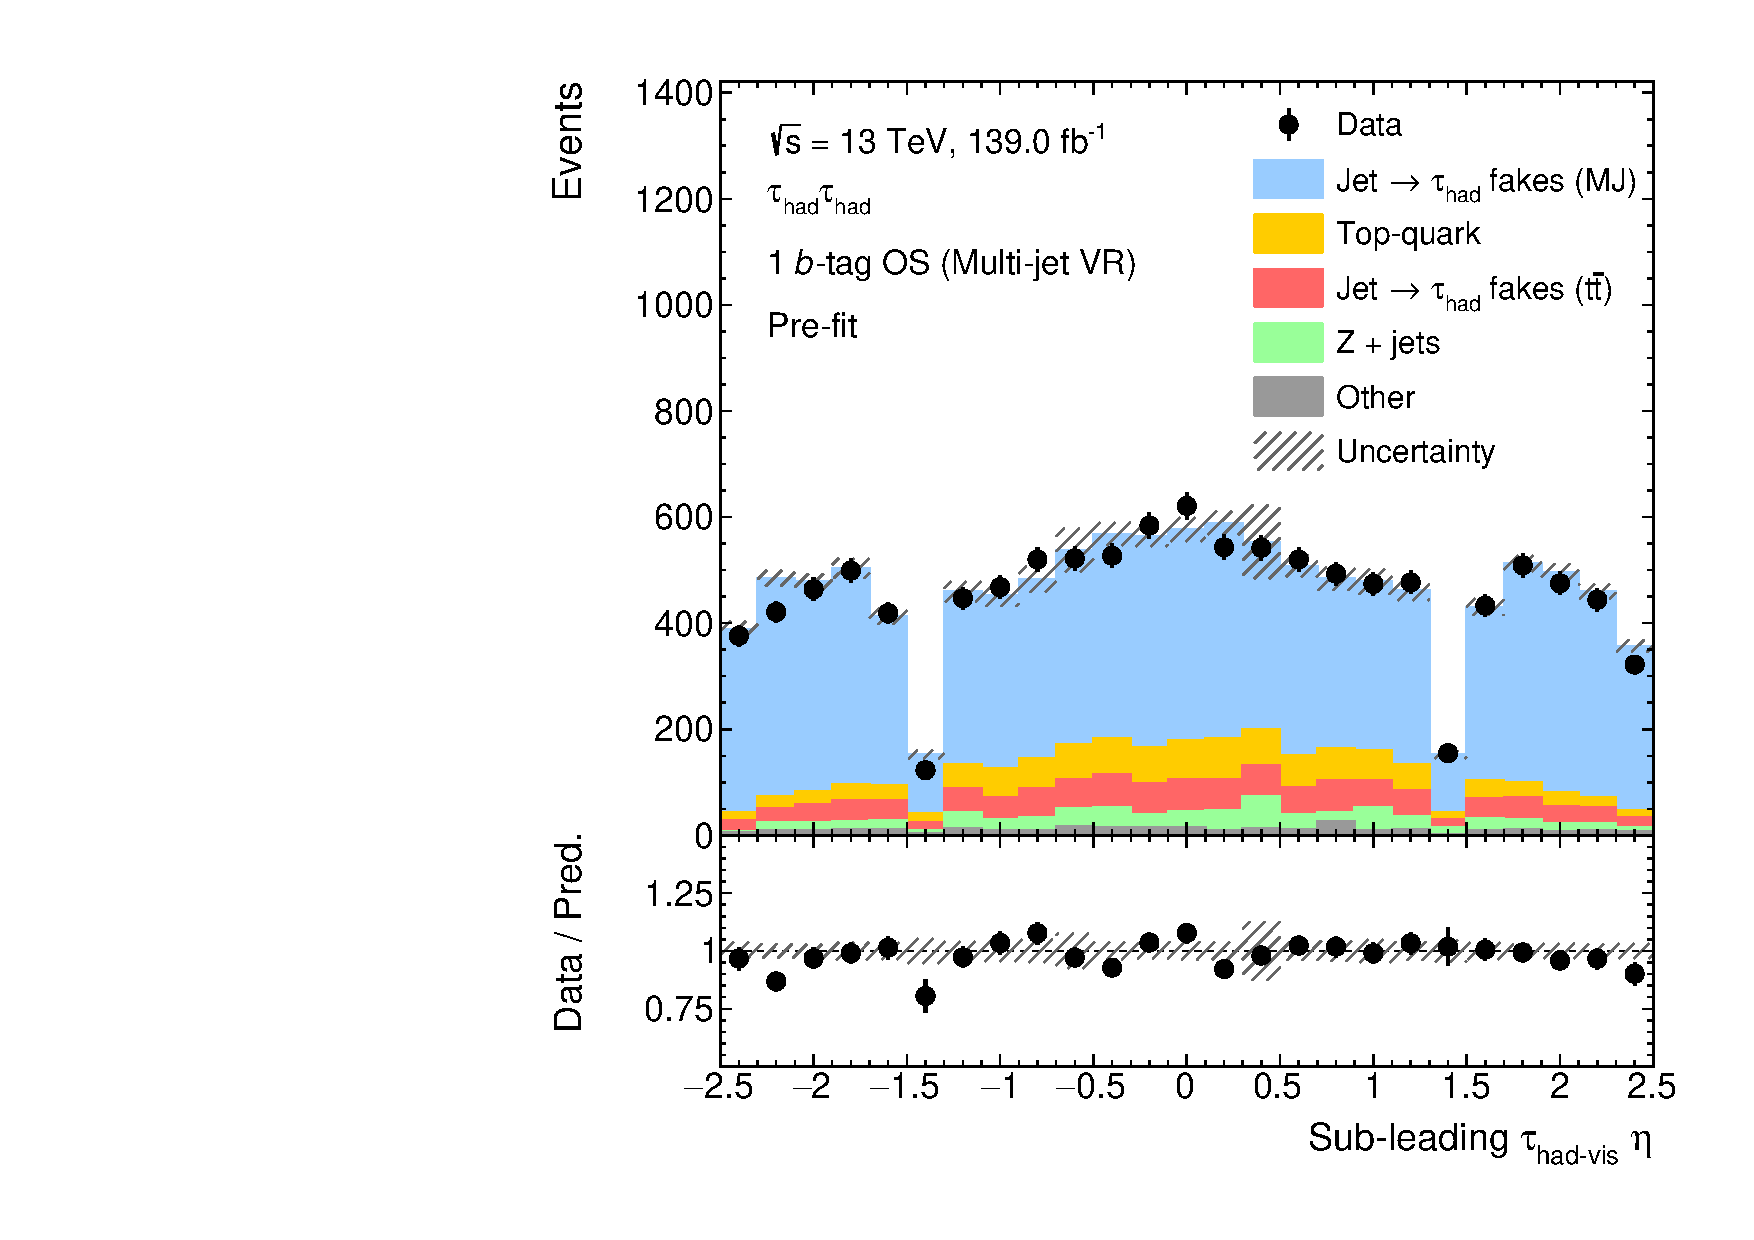
\includegraphics[width=\textwidth]{fakefactors/fake_os_vr/Tau1Eta_fakevr}
  \end{subfigure}

  \begin{subfigure}{0.44\textwidth}
    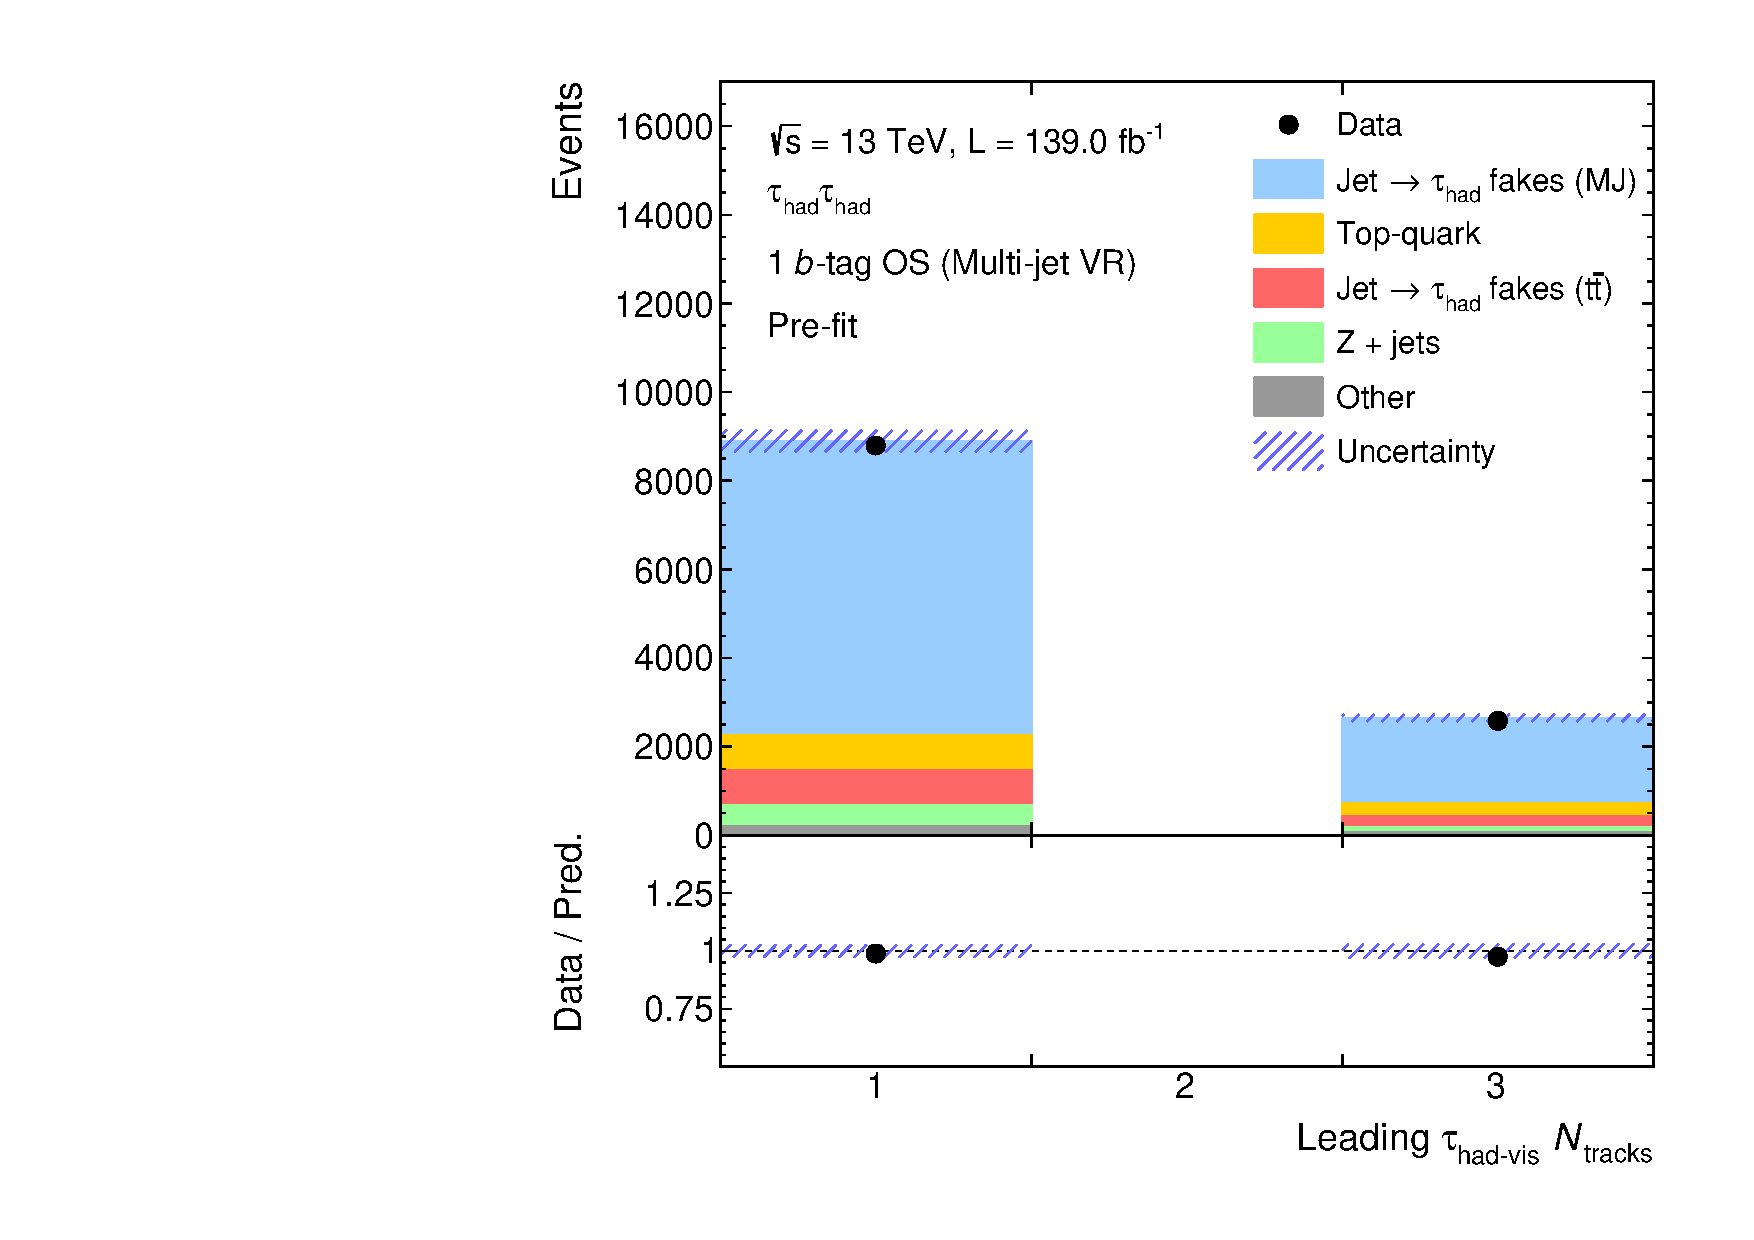
\includegraphics[width=\textwidth]{fakefactors/fake_os_vr/Tau0Ntrk_fakevr}
  \end{subfigure}\hspace*{0.04\textwidth}%
  \begin{subfigure}{0.44\textwidth}
    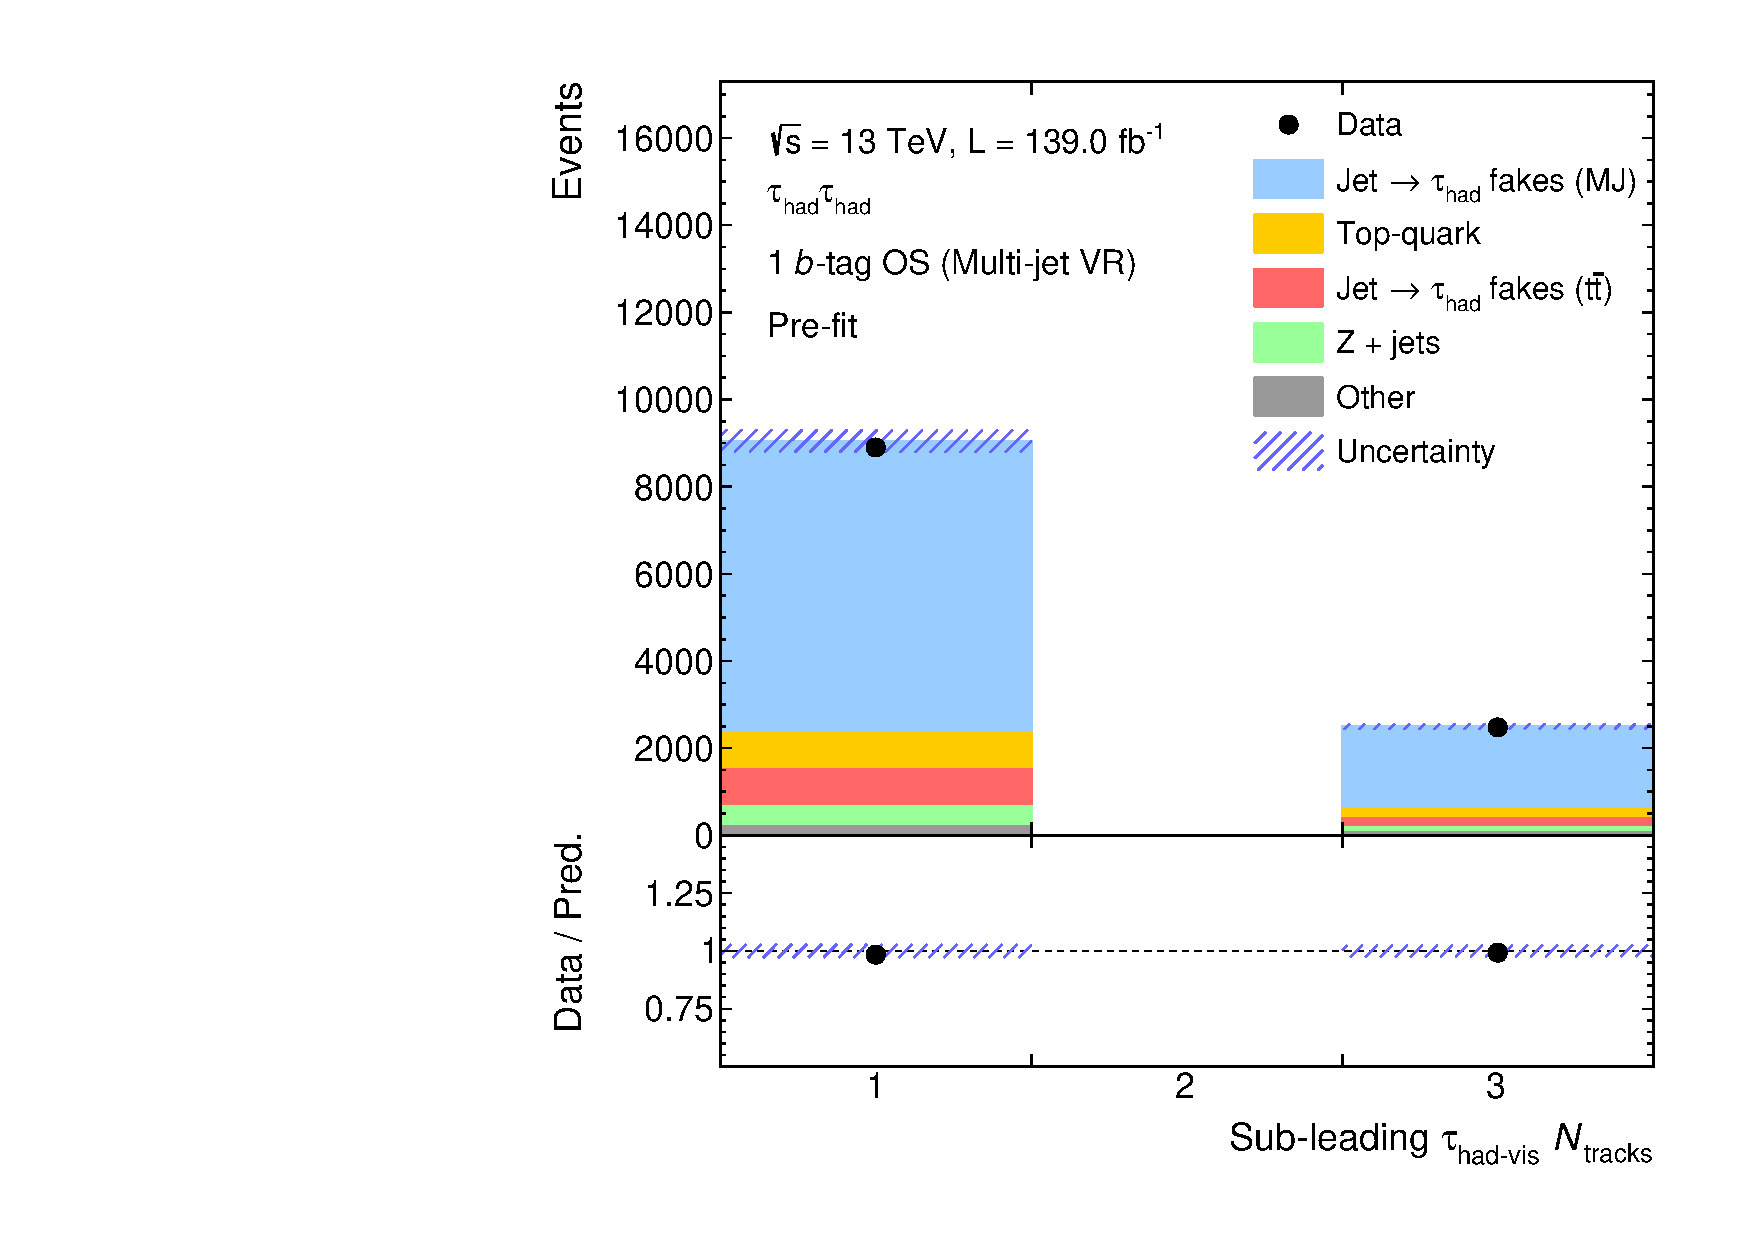
\includegraphics[width=\textwidth]{fakefactors/fake_os_vr/Tau1Ntrk_fakevr}
  \end{subfigure}

  \caption[Distributions of \tauhadvis observables in the multi-jet
  VR.]{Distributions of \tauhadvis observables in the multi-jet VR. The
    multi-jet prediction (blue) is obtained using the FF method. The \tauhadvis
    observables \pT (top), $\eta$ (centre), and $N_{\text{tracks}}$ (bottom) are
    shown for the leading (left) and sub-leading \tauhadvis (right). The
    background prediction is shown pre-fit and includes statistical and
    detector-related systematic uncertainties. No systematic uncertainties on
    the multi-jet estimate are included.}%
  \label{fig:fake_factor_OSVR_kinematics}
\end{figure}

The validity of the FF method can be tested by comparing FFs measured in the
1~$b$-tag~SS~region with FFs obtained from measurements in the
1~$b$-tag~OS~multi-jet~VR. Under the assumptions of the FF method, the OS and SS
FFs are expected to agree. Differences between both sets of FFs can arise from a
violation of the assumptions or from a mismodelling of the subtracted
non-multi-jet backgrounds.

Exemplary comparisons of FFs measured in the OS and SS regions are shown
in~\Cref{fig:fake_factor_OSSS} for DTTs and STTs. A test of the compatibility of
OS and SS FFs for DTTs is tabulated in~\Cref{tab:fake_factor_osss_chi2test},
showing good agreement with one exception. A significant deviation of about
\SI{50}{\percent} between OS and SS FFs is observed for a single FF bin for DTTs
in 2015--2016.\footnote{The FF bin corresponds to 3-prong \tauhadvis candidates
  with \pT from \SIrange{50}{65}{\GeV} in the end-cap of the detector. The OS FF
  for this bin is \num{0.09 +- 0.02} and the SS FF \num{0.21 +- 0.03}.} Except
for this bin and a tension in OS and SS FFs for 3-prong \tauhadvis candidates
selected by STTs, no large differences between OS and SS FFs are observed.
% ; however, the power of this test in detecting differences is limited by the
% large uncertainties on the FF measurement.
To account for non-closure between the OS and SS FFs, the full difference
between both sets of FFs is assigned as an additional systematic uncertainty and
propagated to the multi-jet estimate.

\begin{figure}[htbp]
  \centering

  \begin{subfigure}[t]{0.48\textwidth}
    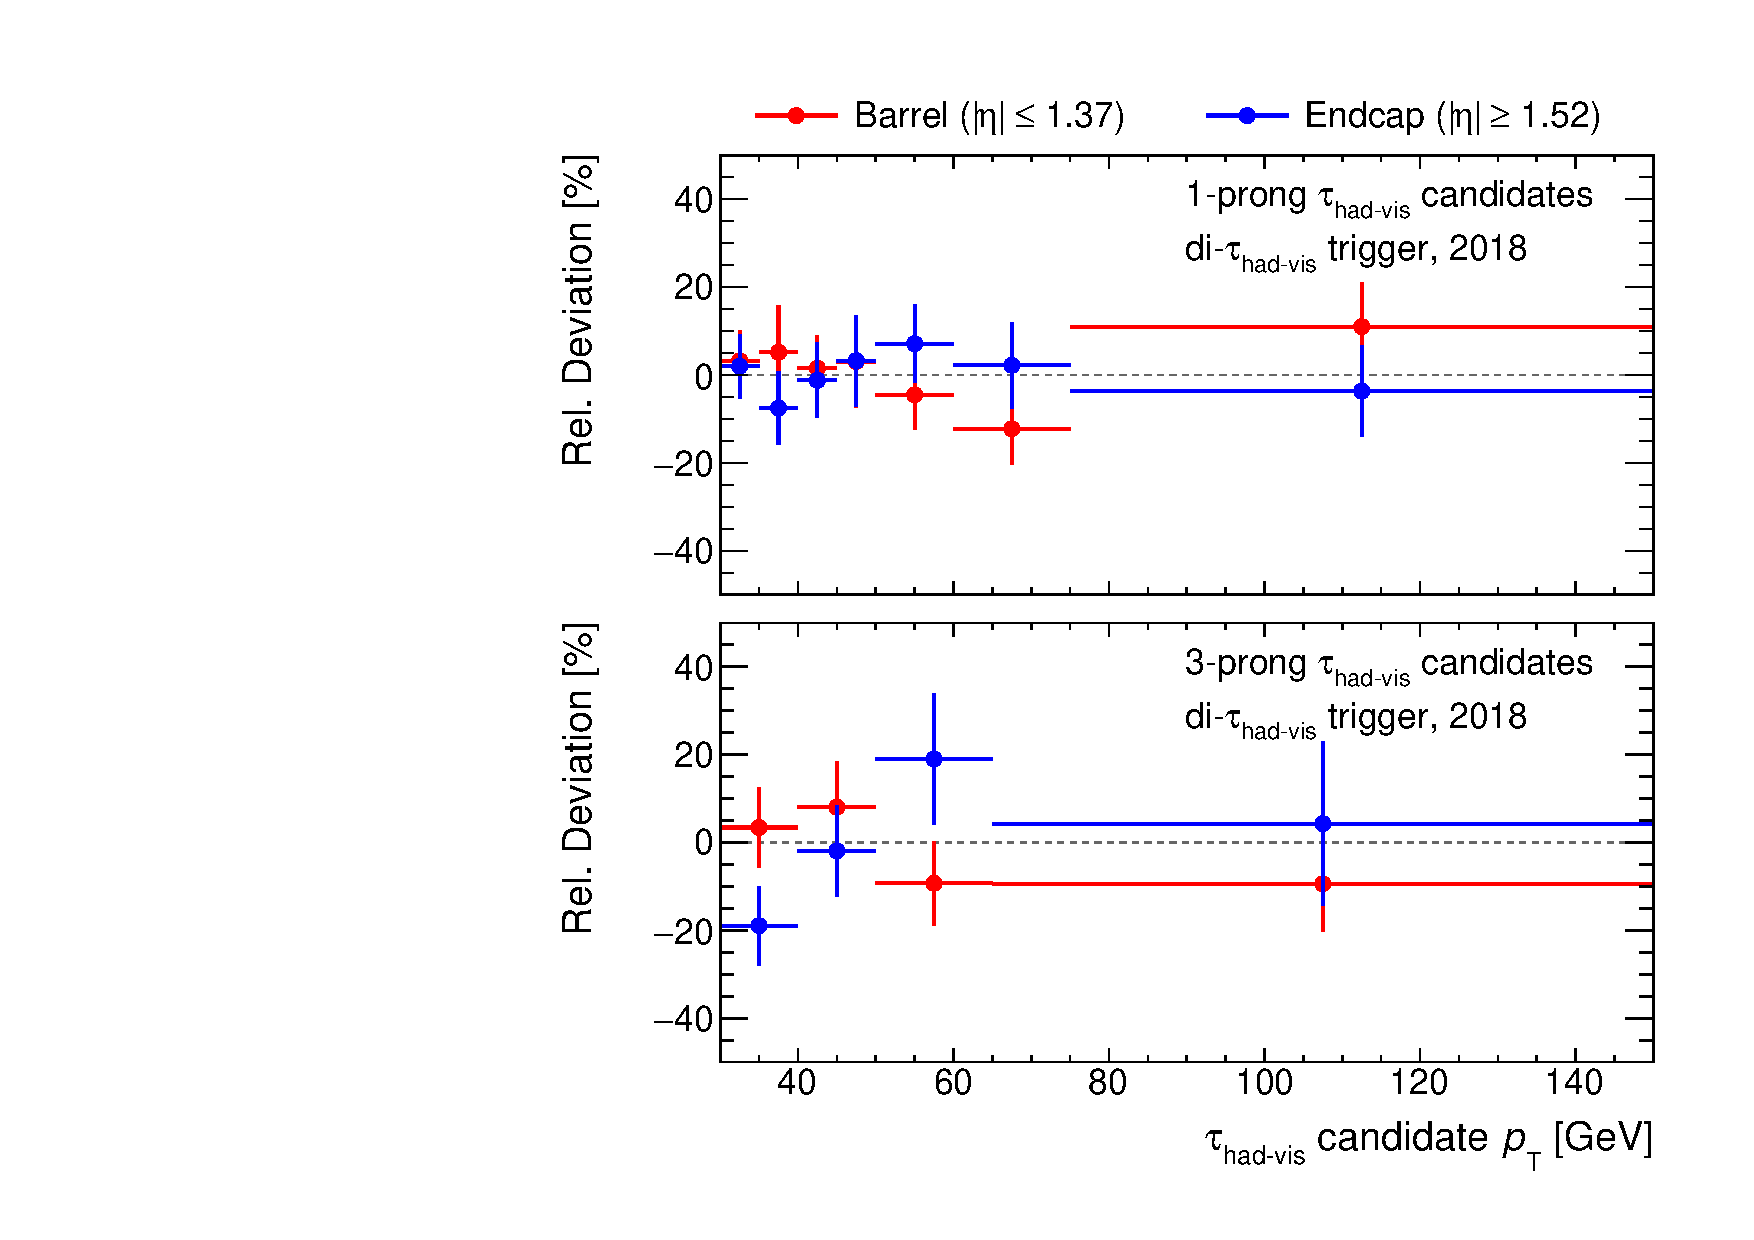
\includegraphics[width=\textwidth]{fakefactors/os_ss/fake_factors_osss_18}
    \subcaption{Comparison of OS and SS FFs for events selected by DTTs. Only
      the 2018 data-taking period.}%
    \label{fig:fake_factor_OSSS_dtt}
  \end{subfigure}\hfill%
  \begin{subfigure}[t]{0.48\textwidth}
    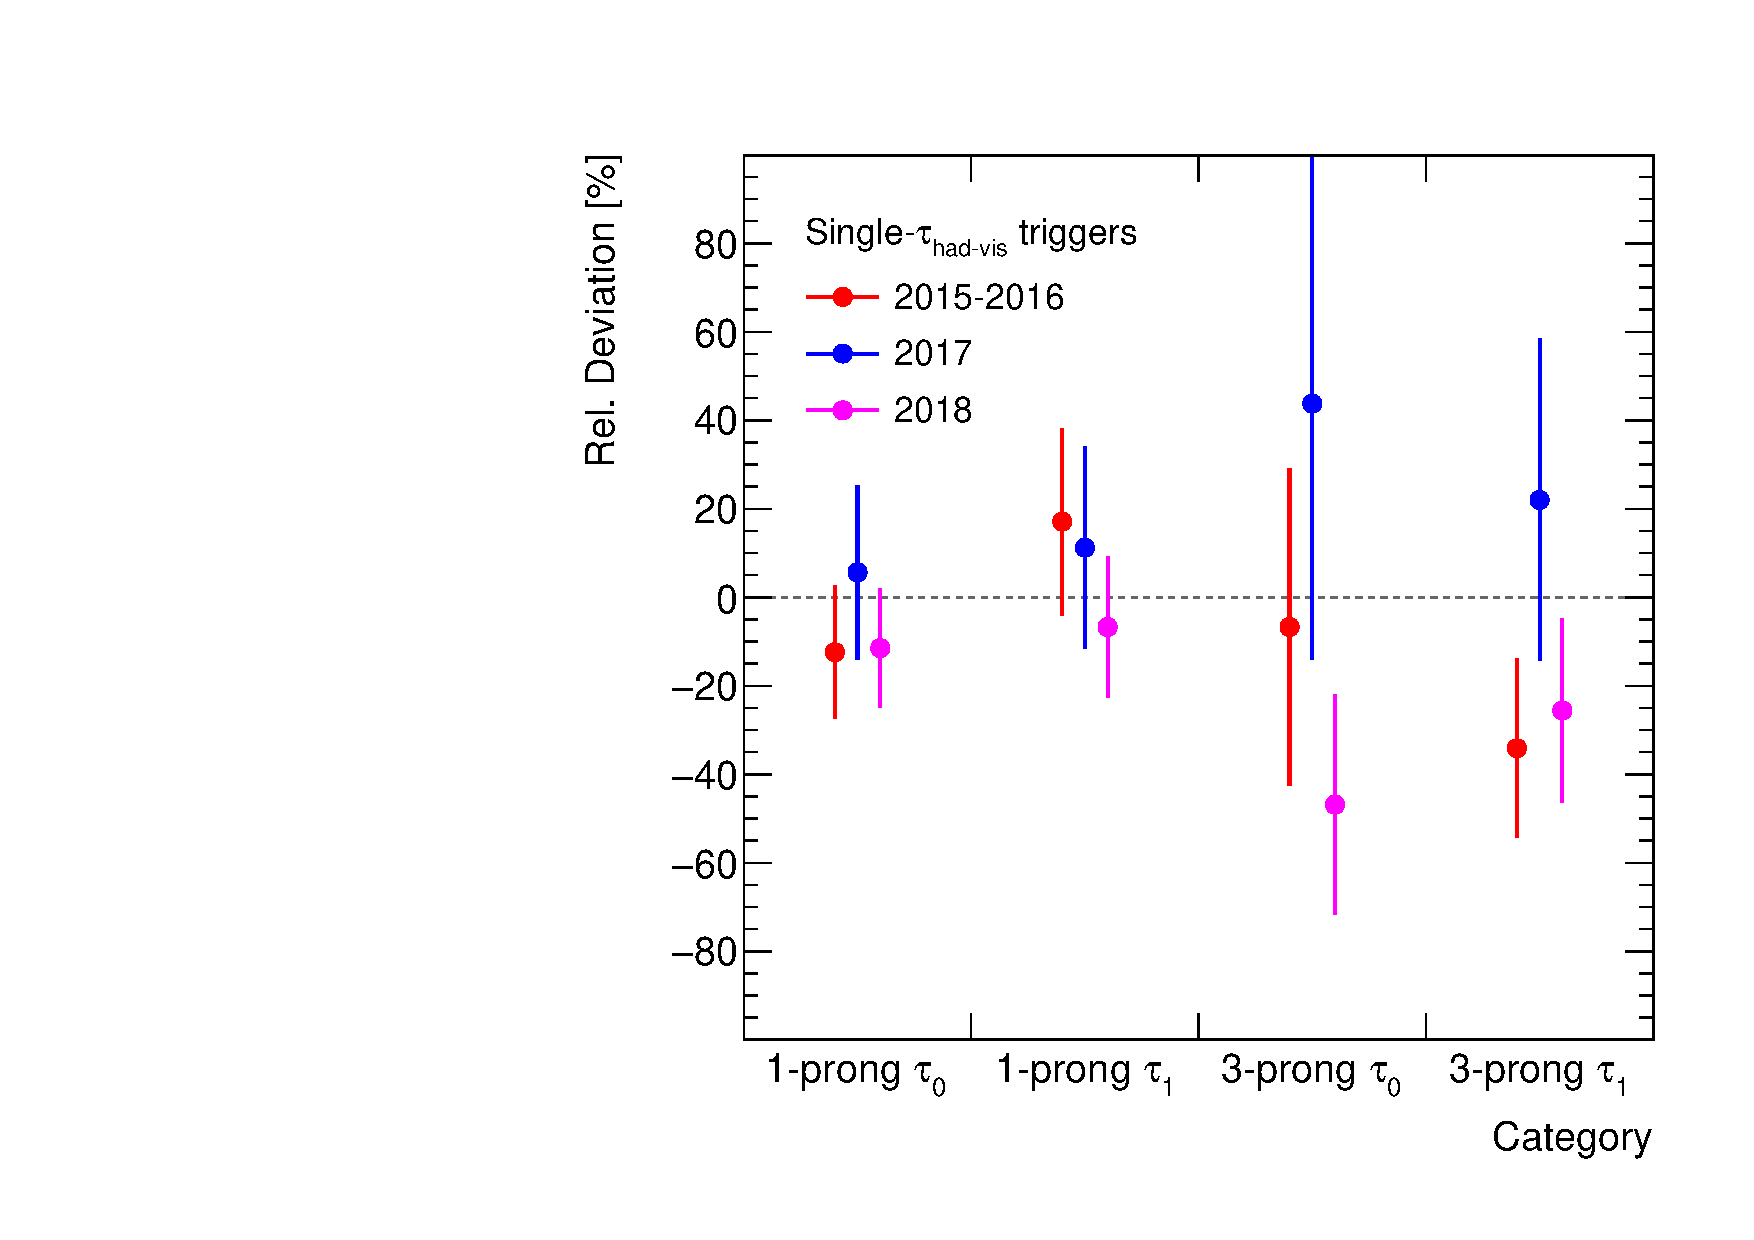
\includegraphics[width=\textwidth]{fakefactors/os_ss/fake_factors_osss_stt}
    \subcaption{Comparison of OS and SS FFs for events selected by STTs for all
      major data-taking periods.}%
    \label{fig:fake_factor_OSSS_stt}
  \end{subfigure}

  \caption[Comparison of OS and SS FFs in the \hadhad channel.]{Relative
    deviation of FFs measured in the 1~$b$-tag~OS multi-jet VR compared to the
    nominal set of FFs measured in the 1~$b$-tag~SS region
    (cf.~\Cref{fig:mjfakes_fake_factors,fig:mjfakes_stt_ffs}). The relative
    deviation is measured as $\FF_\text{OS} / \FF_\text{SS} - 1$ and is used to
    define a non-closure uncertainty that is propagated to the multi-jet
    background estimate when applying SS FFs to events in OS
    regions. Statistical uncertainties from the finite number of observed data
    events and the non-multi-jet subtraction are shown.}%
  \label{fig:fake_factor_OSSS}
\end{figure}

\begin{table}[htbp]
  \centering

  \caption[Comparison of OS and SS FFs for DTT events in the \hadhad
  channel.]{Comparison of OS and SS FFs for DTTs using $\chi^2$-tests to
    summarise the statistical compatibility of both sets of FFs over all
    \tauhadvis \pT bins. The barrel and end-cap detector regions correspond to
    \tauhadvis $|\eta| < 1.37$ and $|\eta| \geq 1.52$, respectively.}%
  \label{tab:fake_factor_osss_chi2test}

  \begin{tabular}{ll@{\hskip 20pt}cr@{\hskip 10pt}|@{\hskip 10pt}cr}
  \toprule
  & & \multicolumn{2}{c}{$\Ntracks = 1$} & \multicolumn{2}{c}{$\Ntracks = 3$} \\
  \cmidrule{3-6}
  {Period} & {Detector region} & {$\chi^2 / \text{NDF}$} & {$p$-value} & {$\chi^2 / \text{NDF}$} & {$p$-value} \\
  \midrule
  \multirow{2}{*}{2015--2016} & Barrel & 4.7 / 7 & \SI{69}{\percent} & \phantom{0}3.7 / 4 & \SI{45}{\percent} \\
                              & Endcap & 7.5 / 7 & \SI{38}{\percent} & 14.8 / 4 & $< \phantom{0}\SI{1}{\percent}$ \\[0.5em]
  \multirow{2}{*}{2017}       & Barrel & 6.1 / 7 & \SI{53}{\percent} & \phantom{0}4.0 / 4 & \SI{41}{\percent} \\
                              & Endcap & 6.2 / 7 & \SI{52}{\percent} & \phantom{0}2.3 / 4 & \SI{68}{\percent} \\[0.5em]
  \multirow{2}{*}{2018}       & Barrel & 4.2 / 7 & \SI{75}{\percent} & \phantom{0}2.3 / 4 & \SI{68}{\percent} \\
                              & Endcap & 1.8 / 7 & \SI{97}{\percent} & \phantom{0}5.7 / 4 & \SI{22}{\percent} \\
  \bottomrule
\end{tabular}


%%% Local Variables:
%%% mode: latex
%%% TeX-master: "../phd_thesis"
%%% End:

\end{table}


\subsubsection{Estimation of Multi-jet Backgrounds in the \hadhad SR}

The multi-jet background in the \hadhad SR (2~$b$-tag~OS~ID) is estimated by
applying FFs from the 1~$b$-tag~SS~region to events in the
2~$b$-tag~OS~Anti-ID~region after subtraction of non-multi-jet processes. In
addition, these FFs are multiplied by a 1~to~2 $b$-tag transfer factor to
account for possible differences between FFs for 1 and 2~$b$-tag regions
(cf.~\Cref{fig:fakefactor_regions}). The change in \btag requirement is not
expected to affect the FFs, such that the transfer factors mainly serve to
provide an estimate of the uncertainty on the extrapolation.

The transfer factors are determined by comparing FFs measured in the
2~$b$-tag~SS~region to ones extracted in the 1~$b$-tag~SS~region. Due to the
large multi-jet rejection of the 2~$b$-tag~requirement, the comparison is
performed using FFs measured inclusively in the trigger category, \tauhadvis \pT
and \tauhadvis $\eta$ but separately for 1- and 3-prong \tauhadvis candidates,
for cases where the anti-\tauhadvis is leading and sub-leading in \pT, and for
the three data-taking periods. The 1 to 2~$b$-tag transfer factor is defined as
the ratio
\begin{align*}
  \text{TF}_{1 \ra 2\,b\text{-tag}} = \frac{\FF_{\text{SS}}^{2\,b\text{-tag}}}{\FF_{\text{SS}}^{1\,b\text{-tag}}} \,\text{.}
\end{align*}
The measured transfer factors are depicted
in~\Cref{fig:mjfakes_transfer_factor}, showing no significant difference between
FFs derived in the 1 and 2 $b$-tag regions. However, the power of this
comparison is limited due to large uncertainties on the FF estimate in the
2~$b$-tag~region. Therefore, extrapolation uncertainties based on the
uncertainties of the transfer factor measurement still have to be assigned.
% Extrapolation uncertainties are defined by varying the transfer factors within
% their uncertainty, separately for every transfer factor bin, propagating the
% effect to the multi-jet estimate in the 2 $b$-tag region.

\begin{figure}[htbp]
  \centering

  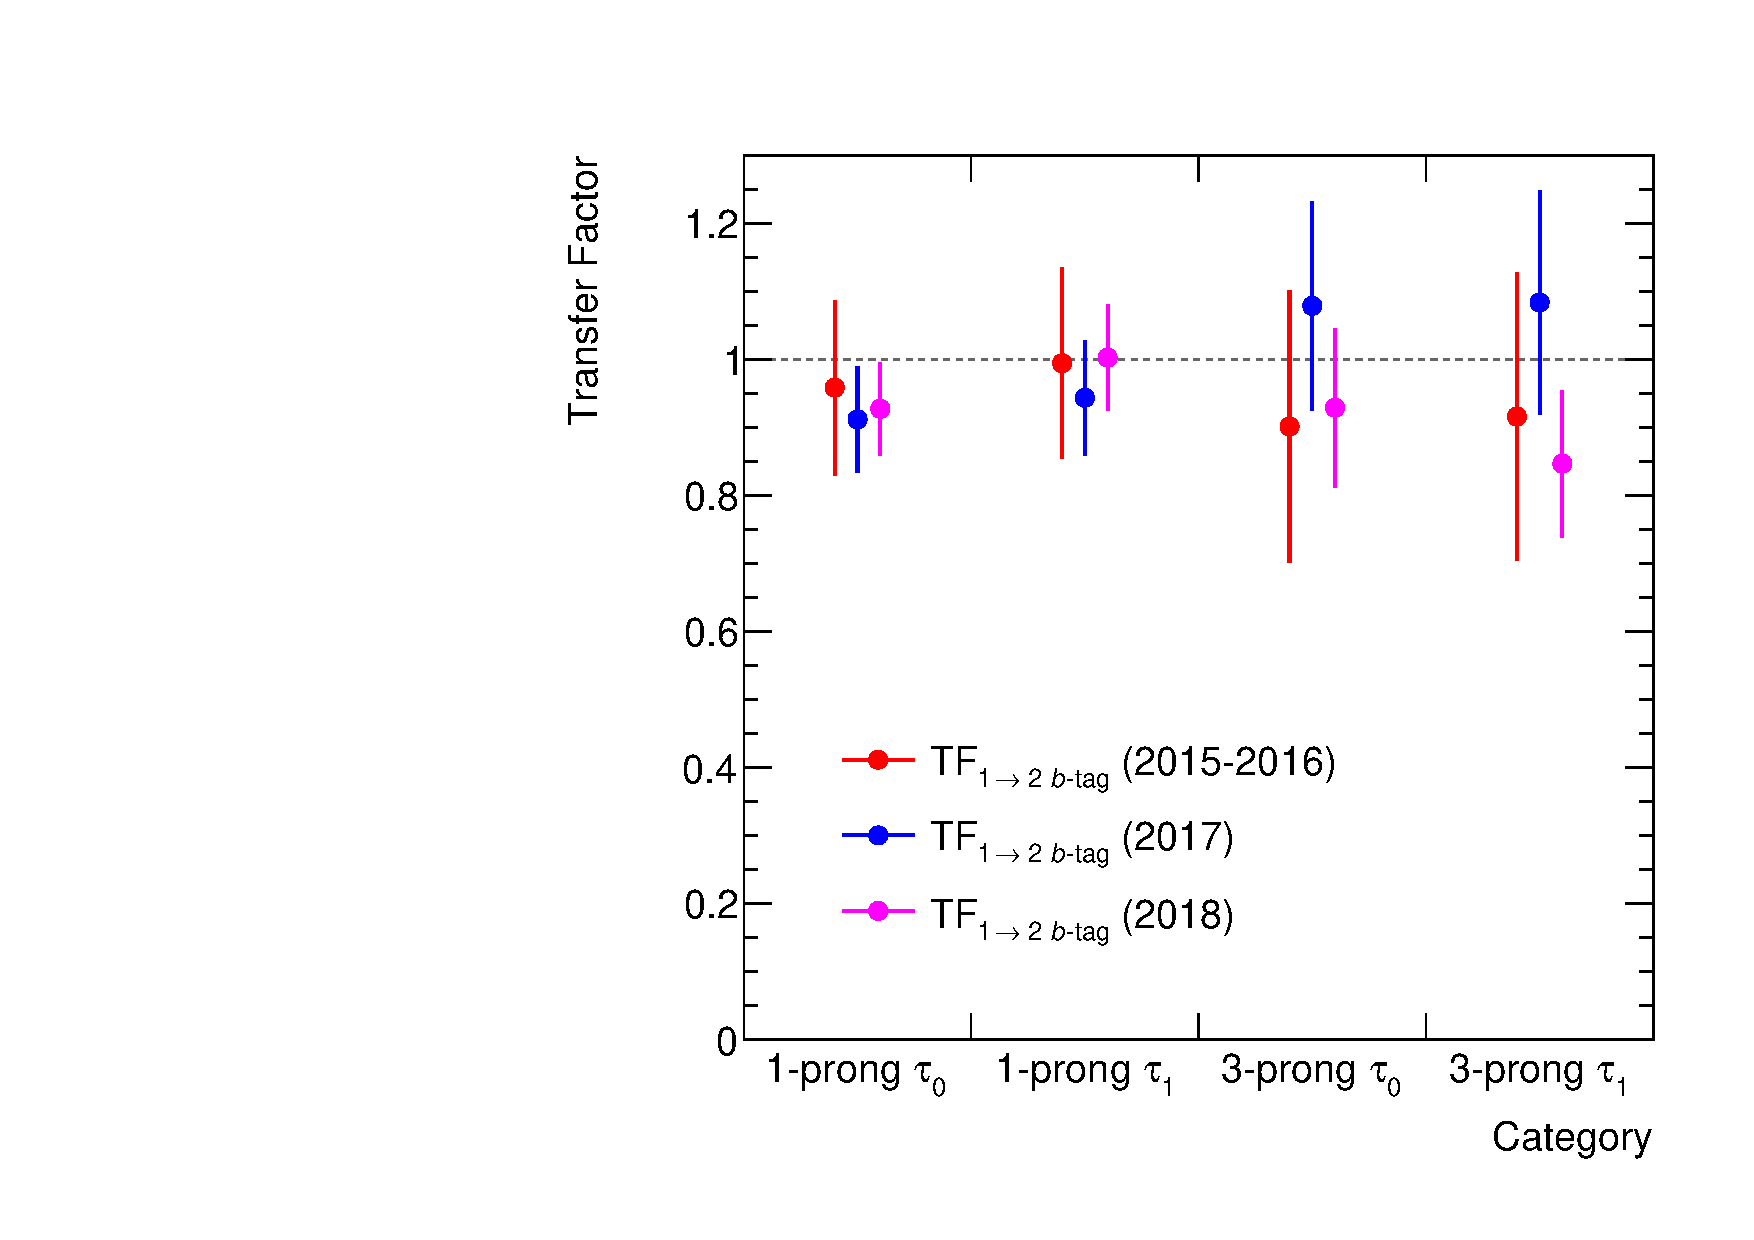
\includegraphics[width=0.495\textwidth]{fakefactors/transfer_factors}

  \caption[Transfer factors for the extrapolation of FFs measured in 1 $b$-tag
  regions to 2 $b$-tag regions.]{Transfer factors for the extrapolation of FFs
    measured in 1 $b$-tag regions to 2 $b$-tag regions. The transfer factors are
    shown separately for 1- and 3-prong \tauhadvis, for cases where the
    anti-\tauhadvis is leading ($\tau_0$) and sub-leading ($\tau_1$) in \pT, and
    for the three major data-taking periods.  The statistical uncertainties on
    the transfer factors are shown.}%
  \label{fig:mjfakes_transfer_factor}
\end{figure}

A disadvantage of applying the FF method in the 2~$b$-tag region is the low
multi-jet purity of about \SI{50}{\percent} in the 2~$b$-tag~OS~Anti-ID~region
(cf.\ \Cref{tab:mjfakes_yields}). Consequently, a large subtraction of
non-multi-jet processes has to be performed when applying FFs to obtain the
multi-jet prediction in the SR.  The size of the subtraction in the
2~$b$-tag~OS~Anti-ID is illustrated in~\Cref{fig:mjfakes_2tag_os_antiid},
showing that \ttbarFakes is the dominant source of non-multi-jet events in this
region. Due to the large relative size of the subtracted non-multi-jet
component, any uncertainties affecting the subtracted components have a large
impact on the multi-jet estimate in the ID region. This is the main limitation
of the multi-jet estimation method used in this analysis.

\begin{figure}[htbp]
  \centering

  \begin{subfigure}{0.49\textwidth}
    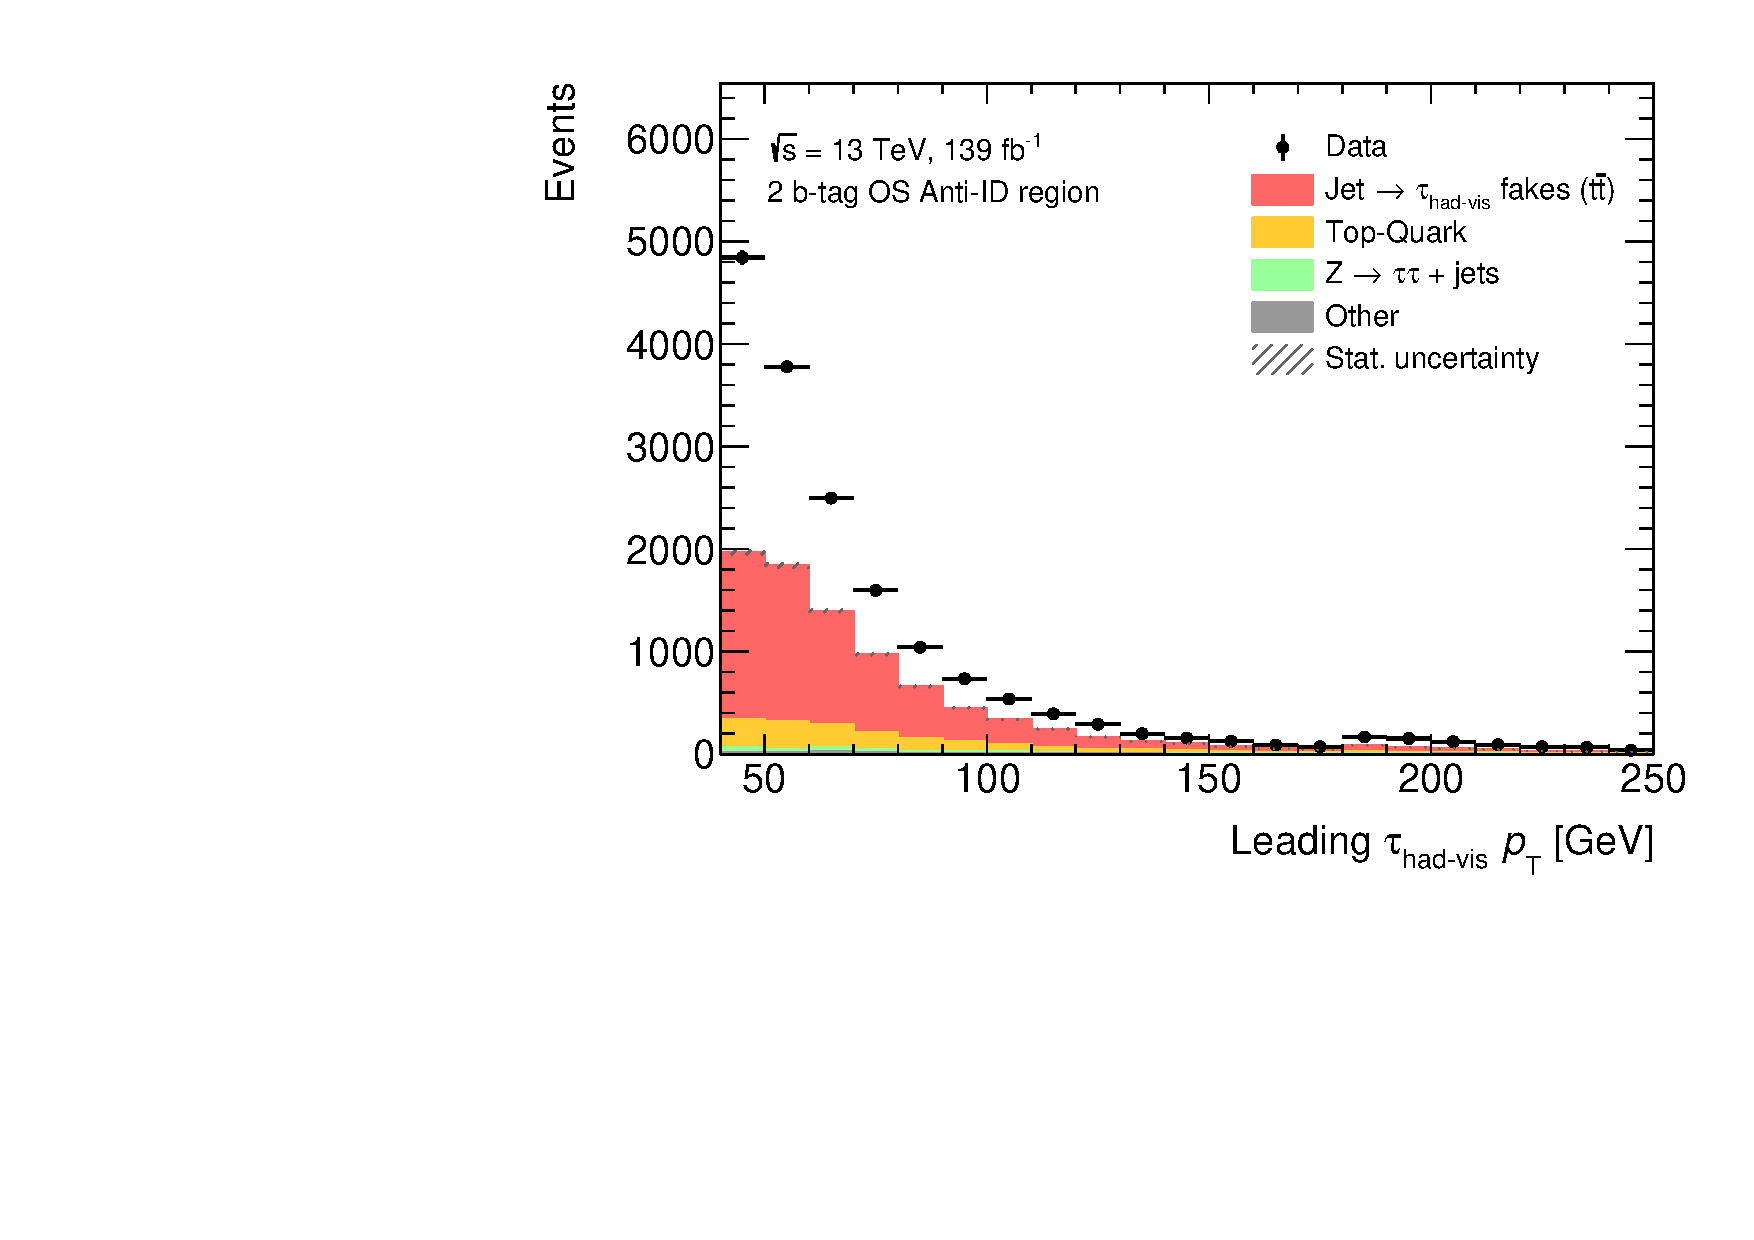
\includegraphics[width=\textwidth]{fakefactors/region_plots/tau0pt_2tag_os_antiid}
    \subcaption{}
  \end{subfigure}%
  \begin{subfigure}{0.49\textwidth}
    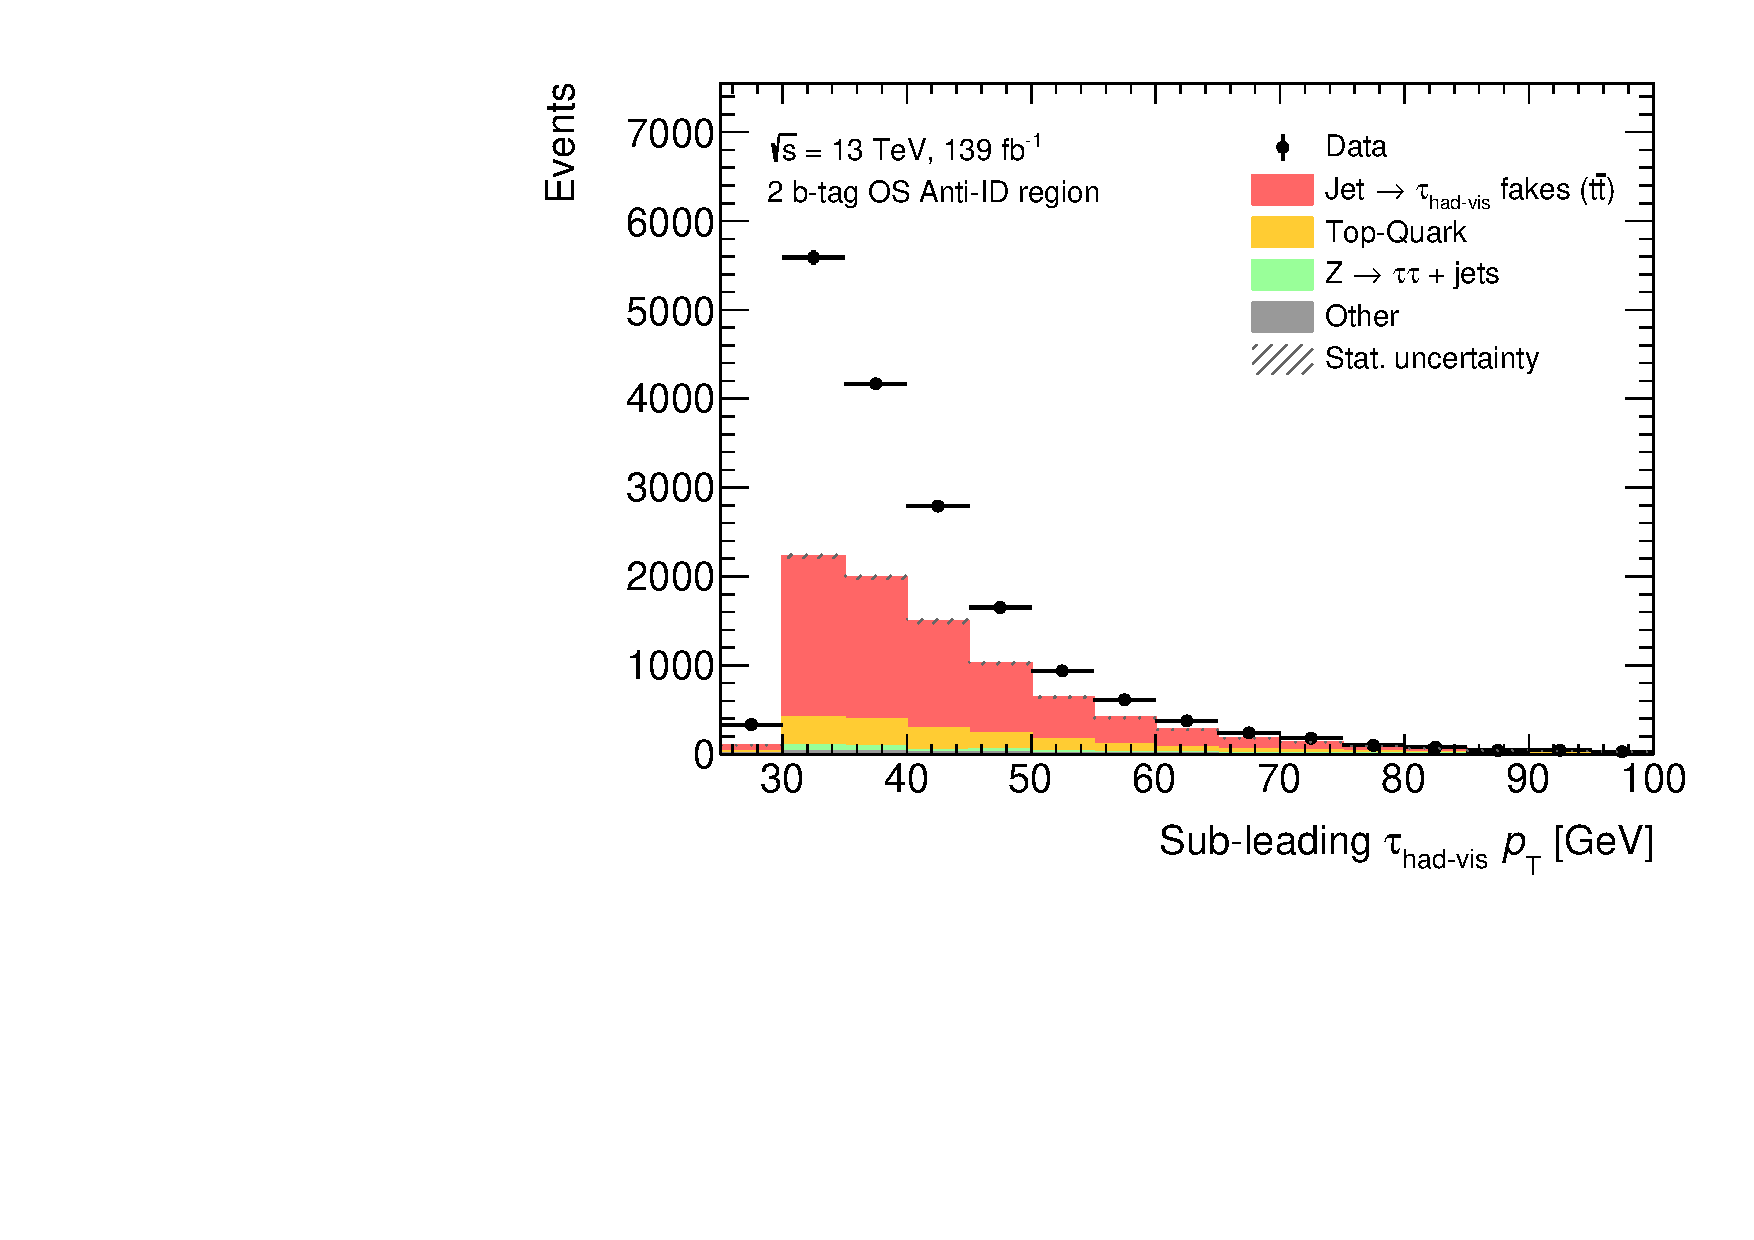
\includegraphics[width=\textwidth]{fakefactors/region_plots/tau1pt_2tag_os_antiid}
    \subcaption{}
  \end{subfigure}

  \caption[Distribution of the leading and sub-leading \tauhadvis candidate \pT
  in the 2 $b$-tag OS Anti-ID region.]{Distribution of the leading (a) and
    sub-leading (b) \tauhadvis candidate \pT in the 2 $b$-tag OS Anti-ID
    region. Non-multi-jet backgrounds are display as coloured histograms and
    include the statistical uncertainty of the prediction. The difference
    between the observed data and the non-multi-jet background prediction is
    attributed to the missing multi-jet estimate.}%
  \label{fig:mjfakes_2tag_os_antiid}
\end{figure}


\subsubsection{Uncertainties on the Multi-jet Prediction in the \hadhad SR}

% Uncertainty ranking:
% ttbarFake subtraction: ~7.4%
% Other subtraction: 5.9%
% Extrapol: ~5.5%
% ttbar subtraction: ~2.8%
% Statistical: 1.9 %
% FF statistical: 1.4%
% OS/SS non-closure: 1.0%
%
% Total: ~11.5%

The following systematic uncertainties are considered and propagated to the
multi-jet estimate in the \hadhad SR:
\begin{itemize}

\item Statistical uncertainties on the FFs.

\item Non-closure uncertainty between FFs estimated in 1~$b$-tag OS and SS
  regions.

\item Uncertainties on the extrapolation of FFs derived in the 1~$b$-tag~region
  to the 2~$b$-tag~region.

\item Uncertainties on the subtraction of \ttbar and other processes in the
  2~$b$-tag OS Anti-ID CR.

\item Statistical uncertainties due to the finite number of events in the
  2~$b$-tag OS Anti-ID CR.

\end{itemize}

% FF measurement statistical uncertainty (1.4%)
The effect of FF statistical uncertainties on the multi-jet prediction in the SR
is estimated by performing variations of FFs separately for all bins of the FF
measurement. The discriminants used in this analysis are insensitive to
variations of FFs in a single bin and therefore all variations are combined into
a single normalisation uncertainty. The resulting uncertainty on the multi-jet
estimate in the SR is~$\pm \SI{1.4}{\percent}$.

% OS-SS uncertainty
The non-closure uncertainty from the comparison of FFs measured in the 1 $b$-tag
SS and OS regions is estimated by assigning the full difference between the
central values of both measurements as an uncertainty on the FFs. The impact of
this variation on the shape of distributions in the SR is taken into account in
the background model. The differences between OS and SS FFs are generally small,
thus the non-closure uncertainty has only a minor impact of
$\pm \SI{1.0}{\percent}$ on the normalisation of the multi-jet estimate.

% Extrapolation uncertainty (varying coherently for all four
% categories)
The uncertainty on the extrapolation of FFs from the 1 $b$-tag to 2 $b$-tag
regions is estimated by performing variations of the transfer factors within
their statistical uncertainties. The variations are performed separately for the
four categories of the transfer factor measurement. In a given category, the
transfer factors for the three data-taking periods are varied coherently.  As a
result, the model of the multi-jet background receives four degrees of freedom
from extrapolation uncertainties and any shape effects of these variations are
propagated to the distributions of interest. The total uncertainty of these
variations on the multi-jet normalisation in the SR is~$\pm \SI{5.5}{\percent}$.

% Subtraction uncertainty
%   ttbar (+16.8% -18.6%)
%   ttbar fakes
%   other (50% up and down)
Systematic uncertainties from the subtraction of non-multi-jet events in the 2
$b$-tag OS Anti-ID region are estimated by performing variations of the
subtracted components. The subtraction of \ttbarTrue, \ttbarFakes, and other
non-multi-jet events is varied separately. In all cases, the effect of the
variations on the shape of the multi-jet prediction in the SR is taken into
account in the model of the multi-jet background.

The uncertainty resulting from the subtraction of \ttbarTrue, which constitutes
about \SI{13}{\percent} of the total subtraction, is obtained by varying the
normalisation of the subtracted \ttbarTrue template by its uncertainty. This
uncertainty is estimated by performing variations of the modelling of \ttbar in
simulation (cf.~\Cref{app:top_uncertainties}). The considered variations and
their impact on the normalisation of the \ttbarTrue template in the 2~$b$-tag OS
Anti-ID region are:
\begin{itemize}
\item Hard scatter and PS+NLO matching: $\pm\SI{6.0}{\percent}$.

\item Parton shower and hadronisation model: $\pm\SI{11}{\percent}$.

\item Renormalisation and factorisation scale:
  $^{\hspace{0.25pt}+\hspace{0.25pt}9.9}_{-9.4}\valuesep{\si{\percent}}$ and
  $^{\hspace{0.25pt}+\hspace{0.25pt}2.8}_{-2.2}\valuesep{\si{\percent}}$.

\item Initial-state and final-state radiation:
  $^{\hspace{0.25pt}+\hspace{0.25pt}0.53}_{-0.68}\valuesep{\si{\percent}}$ and
  $^{\hspace{0.25pt}+\hspace{0.25pt}\phantom{1}5.4}_{-10}\valuesep{\si{\percent}}$.
\end{itemize}
The combination of these sources yields a normalisation uncertainty on the
\ttbarTrue template
of~$^{\hspace{0.25pt}+\hspace{0.25pt}17}_{-19}\valuesep{\si{\percent}}$. Propagating
this uncertainty to the multi-jet prediction in the SR yields an uncertainty
of~$\pm \SI{2.8}{\percent}$. This uncertainty is small due to the small relative
size of the \ttbarTrue subtraction.

The subtraction of \ttbarFakes accounts for \SI{78}{\percent} of the total
non-multi-jet subtraction. The uncertainty on the subtraction of \ttbarFake
events is defined using the \ttbarFakes SF measurement for \antitau previously
described in \Cref{sec:bkg_hadhad_ttbarfakes}. The SF variations explaining most
of the variance of the SF measurement are used to define the \ttbarFakes
subtraction uncertainty, yielding a total of four variations. Other variations
of the measured SFs have negligible impact on the multi-jet prediction and are
therefore omitted to reduce the number of parameters in the background model. An
additional uncertainty is assigned according to the difference between the
\ttbarFakes prediction with and without application of SFs to account for the
reduced set of experimental systematic uncertainties available for the
measurement of \ttbarFakes SF in the Anti-ID region. These five variations have
a combined effect on the normalisation of the multi-jet prediction in the SR
of~$\pm\SI{7.4}{\percent}$.

Other non-multi-jet processes account for approximately \SI{9}{\percent} of the
non-multi-jet subtraction in the 2~$b$-tag OS Anti-ID region. The dominant
contributions are events from \Vjets and single top production, both processes
contributing similarly to the subtraction. As a conservative estimate, the
normalisation of the subtracted components is varied by~$\pm \SI{50}{\percent}$
and propagated to the multi-jet prediction in the SR. This variation changes the
normalisation of the multi-jet estimate in the SR by~$\pm\SI{5.9}{\percent}$.

In addition to these systematic uncertainties, statistical uncertainties
originating from the finite number of events in the 2~$b$-tag OS Anti-ID region
and the statistical precision of the simulation-based subtraction of
non-multi-jet processes are considered. This uncertainty is implemented in the
fit model using the simplified Barlow--Beeston
method~\cite{barlow1993,conway2011}. The effect of this uncertainty on the
multi-jet normalisation in the SR is~$\pm \SI{1.9}{\percent}$.

A summary of all uncertainties affecting the multi-jet background prediction in
the \hadhad~SR is given in~\Cref{tab:multi_jet_uncertainties}. The dominant
sources of uncertainty on the multi-jet normalisation are the subtraction of
\ttbarFakes, the subtraction of other non-multi-jet processes~(\Vjets and single
top), and the extrapolation of 1~$b$-tag FFs to 2~$b$-tag regions. The total
uncertainty on the normalisation of the multi-jet estimate is approximately
\SI{12}{\percent}.

\begin{table}[htbp]
  \centering

  \caption{Uncertainty on the normalisation of the multi-jet background
    prediction in the \hadhad~SR. For a given source of uncertainty, the number
    of independent NPs in the background model is given in the \emph{Components}
    column. Whether a given uncertainty affects the normalisation (N) and/or
    shape (S) of the multi-jet prediction is given in parentheses.
    $\dagger$:~Statistical uncertainties from the finite number of simulated and
    CR events are combined for all background processes.}%
  \label{tab:multi_jet_uncertainties}

  % Nominal fake yield: 1354.7 +- 25.8 (1.9%)
% FF_OSSS__1down                                    +1.0 %
% FF_OSSS__1up                                      -1.0 %
% FF_OTHER_SUBTRACTION__1down                       +5.9 %
% FF_OTHER_SUBTRACTION__1up                         -5.9 %
% FF_TRUE_TTBAR_SUBTRACTION__1down                  +2.8 %
% FF_TRUE_TTBAR_SUBTRACTION__1up                    -2.5 %
% TF_STAT_1P_LEAD__1down                            -3.4 %
% TF_STAT_1P_LEAD__1up                              +3.4 %
% TF_STAT_1P_SUBL__1down                            -3.4 %
% TF_STAT_1P_SUBL__1up                              +3.4 %
% TF_STAT_3P_LEAD__1down                            -1.9 %
% TF_STAT_3P_LEAD__1up                              +1.9 %
% TF_STAT_3P_SUBL__1down                            -1.7 %
% TF_STAT_3P_SUBL__1up                              +1.7 %
% TTBAR_FAKESF_ANTITAU_DIFF__1down                  -2.1 %
% TTBAR_FAKESF_ANTITAU_DIFF__1up                    +2.1 %
% TTBAR_FAKESF_ANTITAU_OFFL_EIGEN0__1down           +0.1 %
% TTBAR_FAKESF_ANTITAU_OFFL_EIGEN0__1up             -0.1 %
% TTBAR_FAKESF_ANTITAU_TAU25EF_EIGEN0__1down        +2.1 %
% TTBAR_FAKESF_ANTITAU_TAU25EF_EIGEN0__1up          -2.2 %
% TTBAR_FAKESF_ANTITAU_TAU25RNN_EIGEN0__1down       +4.9 %
% TTBAR_FAKESF_ANTITAU_TAU25RNN_EIGEN0__1up         -5.1 %
% TTBAR_FAKESF_ANTITAU_TAU25_EIGEN0__1down          +4.2 %
% TTBAR_FAKESF_ANTITAU_TAU25_EIGEN0__1up            -4.3 %
\begin{tabular}{llr}
  \toprule
  \textbf{Source} &  \textbf{Nuisance parameter} & \textbf{Uncertainty}\\
  \midrule
  Statistical uncertainty & --$^\dagger$ & $\pm 1.9\,\%$ \\
  \midrule
  FF statistical uncertainty & \texttt{FF\_STAT\_HADHADSR} & $\pm 1.4\,\%$ \\
  \midrule
  Non-closure of OS / SS FFs & \texttt{FF\_OSSS} & $\pm 1.0\,\%$ \\
  \midrule
  1 to 2 $b$-tag extrapolation & \texttt{TF\_STAT\_1P\_LEAD} & $\pm 3.4\,\%$ \\
                               & \texttt{TF\_STAT\_1P\_SUBL} & $\pm 3.4\,\%$ \\
                               & \texttt{TF\_STAT\_3P\_LEAD} & $\pm 1.9\,\%$ \\
                               & \texttt{TF\_STAT\_3P\_SUBL} & $\pm 1.7\,\%$ \\
  \midrule
  \ttbar subtraction & \texttt{FF\_TRUE\_TTBAR\_SUBTRACTION} & $\pm 2.8\,\%$ \\
  \midrule
  \ttbarFakes subtraction & \texttt{TTBAR\_FAKESF\_ANTITAU\_DIFF} & $\pm 2.1\,\%$ \\
                                 & \texttt{TTBAR\_FAKESF\_ANTITAU\_OFFL\_EIGEN0} & $\pm 0.1\,\%$ \\
                                 & \texttt{TTBAR\_FAKESF\_ANTITAU\_TAU25\_EIGEN0} & $\pm 4.3\,\%$ \\
                                 & \texttt{TTBAR\_FAKESF\_ANTITAU\_TAU25EF\_EIGEN0} & $\pm 2.2\,\%$ \\
                                 & \texttt{TTBAR\_FAKESF\_ANTITAU\_TAU25RNN\_EIGEN0} & $\pm 5.1\,\%$ \\
  \midrule
  Other subtraction & \texttt{FF\_OTHER\_SUBTRACTION} & $\pm 5.9\,\%$ \\
  \bottomrule
\end{tabular}

%%% Local Variables:
%%% mode: latex
%%% TeX-master: "../phd_thesis"
%%% End:

\end{table}


%%% Local Variables:
%%% mode: latex
%%% TeX-master: "../../phd_thesis"
%%% End:
